
%% bare_jrnl.tex
%% V1.4b
%% 2015/08/26
%% by Michael Shell
%% see http://www.michaelshell.org/
%% for current contact information.
%%
%% This is a skeleton file demonstrating the use of IEEEtran.cls
%% (requires IEEEtran.cls version 1.8b or later) with an IEEE
%% journal paper.
%%
%% Support sites:
%% http://www.michaelshell.org/tex/ieeetran/
%% http://www.ctan.org/pkg/ieeetran
%% and
%% http://www.ieee.org/

%%*************************************************************************
%% Legal Notice:
%% This code is offered as-is without any warranty either expressed or
%% implied; without even the implied warranty of MERCHANTABILITY or
%% FITNESS FOR A PARTICULAR PURPOSE! 
%% User assumes all risk.
%% In no event shall the IEEE or any contributor to this code be liable for
%% any damages or losses, including, but not limited to, incidental,
%% consequential, or any other damages, resulting from the use or misuse
%% of any information contained here.
%%
%% All comments are the opinions of their respective authors and are not
%% necessarily endorsed by the IEEE.
%%
%% This work is distributed under the LaTeX Project Public License (LPPL)
%% ( http://www.latex-project.org/ ) version 1.3, and may be freely used,
%% distributed and modified. A copy of the LPPL, version 1.3, is included
%% in the base LaTeX documentation of all distributions of LaTeX released
%% 2003/12/01 or later.
%% Retain all contribution notices and credits.
%% ** Modified files should be clearly indicated as such, including  **
%% ** renaming them and changing author support contact information. **
%%*************************************************************************


% *** Authors should verify (and, if needed, correct) their LaTeX system  ***
% *** with the testflow diagnostic prior to trusting their LaTeX platform ***
% *** with production work. The IEEE's font choices and paper sizes can   ***
% *** trigger bugs that do not appear when using other class files.       ***                          ***
% The testflow support page is at:
% http://www.michaelshell.org/tex/testflow/



\documentclass[journal]{IEEEtran}
%
% If IEEEtran.cls has not been installed into the LaTeX system files,
% manually specify the path to it like:
% \documentclass[journal]{../sty/IEEEtran}





% Some very useful LaTeX packages include:
% (uncomment the ones you want to load)


% *** MISC UTILITY PACKAGES ***
%
%\usepackage{ifpdf}
% Heiko Oberdiek's ifpdf.sty is very useful if you need conditional
% compilation based on whether the output is pdf or dvi.
% usage:
% \ifpdf
%   % pdf code
% \else
%   % dvi code
% \fi
% The latest version of ifpdf.sty can be obtained from:
% http://www.ctan.org/pkg/ifpdf
% Also, note that IEEEtran.cls V1.7 and later provides a builtin
% \ifCLASSINFOpdf conditional that works the same way.
% When switching from latex to pdflatex and vice-versa, the compiler may
% have to be run twice to clear warning/error messages.






% *** CITATION PACKAGES ***
%
\usepackage{cite}
% cite.sty was written by Donald Arseneau
% V1.6 and later of IEEEtran pre-defines the format of the cite.sty package
% \cite{} output to follow that of the IEEE. Loading the cite package will
% result in citation numbers being automatically sorted and properly
% "compressed/ranged". e.g., [1], [9], [2], [7], [5], [6] without using
% cite.sty will become [1], [2], [5]--[7], [9] using cite.sty. cite.sty's
% \cite will automatically add leading space, if needed. Use cite.sty's
% noadjust option (cite.sty V3.8 and later) if you want to turn this off
% such as if a citation ever needs to be enclosed in parenthesis.
% cite.sty is already installed on most LaTeX systems. Be sure and use
% version 5.0 (2009-03-20) and later if using hyperref.sty.
% The latest version can be obtained at:
% http://www.ctan.org/pkg/cite
% The documentation is contained in the cite.sty file itself.



% \usepackage{cite}
% \usepackage{amsmath,amssymb,amsfonts}
% \usepackage{algorithmic}
% \usepackage{graphicx}
% \usepackage{textcomp}
% \usepackage{xcolor}


% *** GRAPHICS RELATED PACKAGES ***
%
\ifCLASSINFOpdf
   \usepackage[pdftex]{graphicx}
  % declare the path(s) where your graphic files are
  % \graphicspath{{../pdf/}{../jpeg/}}
  % and their extensions so you won't have to specify these with
  % every instance of \includegraphics
  % \DeclareGraphicsExtensions{.pdf,.jpeg,.png}
\else
  % or other class option (dvipsone, dvipdf, if not using dvips). graphicx
  % will default to the driver specified in the system graphics.cfg if no
  % driver is specified.
   \usepackage[dvips]{graphicx}
  % declare the path(s) where your graphic files are
  % \graphicspath{{../eps/}}
  % and their extensions so you won't have to specify these with
  % every instance of \includegraphics
  % \DeclareGraphicsExtensions{.eps}
\fi
% graphicx was written by David Carlisle and Sebastian Rahtz. It is
% required if you want graphics, photos, etc. graphicx.sty is already
% installed on most LaTeX systems. The latest version and documentation
% can be obtained at: 
% http://www.ctan.org/pkg/graphicx
% Another good source of documentation is "Using Imported Graphics in
% LaTeX2e" by Keith Reckdahl which can be found at:
% http://www.ctan.org/pkg/epslatex
%
% latex, and pdflatex in dvi mode, support graphics in encapsulated
% postscript (.eps) format. pdflatex in pdf mode supports graphics
% in .pdf, .jpeg, .png and .mps (metapost) formats. Users should ensure
% that all non-photo figures use a vector format (.eps, .pdf, .mps) and
% not a bitmapped formats (.jpeg, .png). The IEEE frowns on bitmapped formats
% which can result in "jaggedy"/blurry rendering of lines and letters as
% well as large increases in file sizes.
%
% You can find documentation about the pdfTeX application at:
% http://www.tug.org/applications/pdftex





% *** MATH PACKAGES ***
%
\usepackage{amsmath,amssymb,amsfonts}
% A popular package from the American Mathematical Society that provides
% many useful and powerful commands for dealing with mathematics.
%
% Note that the amsmath package sets \interdisplaylinepenalty to 10000
% thus preventing page breaks from occurring within multiline equations. Use:
%\interdisplaylinepenalty=2500
% after loading amsmath to restore such page breaks as IEEEtran.cls normally
% does. amsmath.sty is already installed on most LaTeX systems. The latest
% version and documentation can be obtained at:
% http://www.ctan.org/pkg/amsmath





% *** SPECIALIZED LIST PACKAGES ***
%
\usepackage{algorithmic}
% algorithmic.sty was written by Peter Williams and Rogerio Brito.
% This package provides an algorithmic environment fo describing algorithms.
% You can use the algorithmic environment in-text or within a figure
% environment to provide for a floating algorithm. Do NOT use the algorithm
% floating environment provided by algorithm.sty (by the same authors) or
% algorithm2e.sty (by Christophe Fiorio) as the IEEE does not use dedicated
% algorithm float types and packages that provide these will not provide
% correct IEEE style captions. The latest version and documentation of
% algorithmic.sty can be obtained at:
% http://www.ctan.org/pkg/algorithms
% Also of interest may be the (relatively newer and more customizable)
% algorithmicx.sty package by Szasz Janos:
% http://www.ctan.org/pkg/algorithmicx




% *** ALIGNMENT PACKAGES ***
%
%\usepackage{array}
% Frank Mittelbach's and David Carlisle's array.sty patches and improves
% the standard LaTeX2e array and tabular environments to provide better
% appearance and additional user controls. As the default LaTeX2e table
% generation code is lacking to the point of almost being broken with
% respect to the quality of the end results, all users are strongly
% advised to use an enhanced (at the very least that provided by array.sty)
% set of table tools. array.sty is already installed on most systems. The
% latest version and documentation can be obtained at:
% http://www.ctan.org/pkg/array


% IEEEtran contains the IEEEeqnarray family of commands that can be used to
% generate multiline equations as well as matrices, tables, etc., of high
% quality.




% *** SUBFIGURE PACKAGES ***
\ifCLASSOPTIONcompsoc
 \usepackage[caption=false,font=normalsize,labelfont=sf,textfont=sf]{subfig}
\else
 \usepackage[caption=false,font=footnotesize]{subfig}
\fi
% subfig.sty, written by Steven Douglas Cochran, is the modern replacement
% for subfigure.sty, the latter of which is no longer maintained and is
% incompatible with some LaTeX packages including fixltx2e. However,
% subfig.sty requires and automatically loads Axel Sommerfeldt's caption.sty
% which will override IEEEtran.cls' handling of captions and this will result
% in non-IEEE style figure/table captions. To prevent this problem, be sure
% and invoke subfig.sty's "caption=false" package option (available since
% subfig.sty version 1.3, 2005/06/28) as this is will preserve IEEEtran.cls
% handling of captions.
% Note that the Computer Society format requires a larger sans serif font
% than the serif footnote size font used in traditional IEEE formatting
% and thus the need to invoke different subfig.sty package options depending
% on whether compsoc mode has been enabled.
%
% The latest version and documentation of subfig.sty can be obtained at:
% http://www.ctan.org/pkg/subfig




% *** FLOAT PACKAGES ***
%
%\usepackage{fixltx2e}
% fixltx2e, the successor to the earlier fix2col.sty, was written by
% Frank Mittelbach and David Carlisle. This package corrects a few problems
% in the LaTeX2e kernel, the most notable of which is that in current
% LaTeX2e releases, the ordering of single and double column floats is not
% guaranteed to be preserved. Thus, an unpatched LaTeX2e can allow a
% single column figure to be placed prior to an earlier double column
% figure.
% Be aware that LaTeX2e kernels dated 2015 and later have fixltx2e.sty's
% corrections already built into the system in which case a warning will
% be issued if an attempt is made to load fixltx2e.sty as it is no longer
% needed.
% The latest version and documentation can be found at:
% http://www.ctan.org/pkg/fixltx2e


%\usepackage{stfloats}
% stfloats.sty was written by Sigitas Tolusis. This package gives LaTeX2e
% the ability to do double column floats at the bottom of the page as well
% as the top. (e.g., "\begin{figure*}[!b]" is not normally possible in
% LaTeX2e). It also provides a command:
%\fnbelowfloat
% to enable the placement of footnotes below bottom floats (the standard
% LaTeX2e kernel puts them above bottom floats). This is an invasive package
% which rewrites many portions of the LaTeX2e float routines. It may not work
% with other packages that modify the LaTeX2e float routines. The latest
% version and documentation can be obtained at:
% http://www.ctan.org/pkg/stfloats
% Do not use the stfloats baselinefloat ability as the IEEE does not allow
% \baselineskip to stretch. Authors submitting work to the IEEE should note
% that the IEEE rarely uses double column equations and that authors should try
% to avoid such use. Do not be tempted to use the cuted.sty or midfloat.sty
% packages (also by Sigitas Tolusis) as the IEEE does not format its papers in
% such ways.
% Do not attempt to use stfloats with fixltx2e as they are incompatible.
% Instead, use Morten Hogholm'a dblfloatfix which combines the features
% of both fixltx2e and stfloats:
%
% \usepackage{dblfloatfix}
% The latest version can be found at:
% http://www.ctan.org/pkg/dblfloatfix




%\ifCLASSOPTIONcaptionsoff
%  \usepackage[nomarkers]{endfloat}
% \let\MYoriglatexcaption\caption
% \renewcommand{\caption}[2][\relax]{\MYoriglatexcaption[#2]{#2}}
%\fi
% endfloat.sty was written by James Darrell McCauley, Jeff Goldberg and 
% Axel Sommerfeldt. This package may be useful when used in conjunction with 
% IEEEtran.cls'  captionsoff option. Some IEEE journals/societies require that
% submissions have lists of figures/tables at the end of the paper and that
% figures/tables without any captions are placed on a page by themselves at
% the end of the document. If needed, the draftcls IEEEtran class option or
% \CLASSINPUTbaselinestretch interface can be used to increase the line
% spacing as well. Be sure and use the nomarkers option of endfloat to
% prevent endfloat from "marking" where the figures would have been placed
% in the text. The two hack lines of code above are a slight modification of
% that suggested by in the endfloat docs (section 8.4.1) to ensure that
% the full captions always appear in the list of figures/tables - even if
% the user used the short optional argument of \caption[]{}.
% IEEE papers do not typically make use of \caption[]'s optional argument,
% so this should not be an issue. A similar trick can be used to disable
% captions of packages such as subfig.sty that lack options to turn off
% the subcaptions:
% For subfig.sty:
% \let\MYorigsubfloat\subfloat
% \renewcommand{\subfloat}[2][\relax]{\MYorigsubfloat[]{#2}}
% However, the above trick will not work if both optional arguments of
% the \subfloat command are used. Furthermore, there needs to be a
% description of each subfigure *somewhere* and endfloat does not add
% subfigure captions to its list of figures. Thus, the best approach is to
% avoid the use of subfigure captions (many IEEE journals avoid them anyway)
% and instead reference/explain all the subfigures within the main caption.
% The latest version of endfloat.sty and its documentation can obtained at:
% http://www.ctan.org/pkg/endfloat
%
% The IEEEtran \ifCLASSOPTIONcaptionsoff conditional can also be used
% later in the document, say, to conditionally put the References on a 
% page by themselves.




% *** PDF, URL AND HYPERLINK PACKAGES ***
%
%\usepackage{url}
% url.sty was written by Donald Arseneau. It provides better support for
% handling and breaking URLs. url.sty is already installed on most LaTeX
% systems. The latest version and documentation can be obtained at:
% http://www.ctan.org/pkg/url
% Basically, \url{my_url_here}.




% *** Do not adjust lengths that control margins, column widths, etc. ***
% *** Do not use packages that alter fonts (such as pslatex).         ***
% There should be no need to do such things with IEEEtran.cls V1.6 and later.
% (Unless specifically asked to do so by the journal or conference you plan
% to submit to, of course. )


% correct bad hyphenation here
\hyphenation{op-tical net-works semi-conduc-tor}


\begin{document}
%
% paper title
% Titles are generally capitalized except for words such as a, an, and, as,
% at, but, by, for, in, nor, of, on, or, the, to and up, which are usually
% not capitalized unless they are the first or last word of the title.
% Linebreaks \\ can be used within to get better formatting as desired.
% Do not put math or special symbols in the title.
\title{Towards Designer Modeling through \\Design Style Clustering}
\title{Designer Modeling through Design Style Clustering}
%
%
% author names and IEEE memberships
% note positions of commas and nonbreaking spaces ( ~ ) LaTeX will not break
% a structure at a ~ so this keeps an author's name from being broken across
% two lines.
% use \thanks{} to gain access to the first footnote area
% a separate \thanks must be used for each paragraph as LaTeX2e's \thanks
% was not built to handle multiple paragraphs
%

% \author{Michael~Shell,~\IEEEmembership{Member,~IEEE,}
%         John~Doe,~\IEEEmembership{Fellow,~OSA,}
%         and~Jane~Doe,~\IEEEmembership{Life~Fellow,~IEEE}% <-this % stops a space
% \thanks{M. Shell was with the Department
% of Electrical and Computer Engineering, Georgia Institute of Technology, Atlanta,
% GA, 30332 USA e-mail: (see http://www.michaelshell.org/contact.html).}% <-this % stops a space
% \thanks{J. Doe and J. Doe are with Anonymous University.}% <-this % stops a space
% \thanks{Manuscript received April 19, 2005; revised August 26, 2015.}}

\author{Alberto~Alvarez,
        Jose~Font,
        and~Julian~Togelius,~\IEEEmembership{Member,~IEEE}% <-this % stops a space
\thanks{A. Alvarez, and J. Font are with the Department of Computer Science and Media Technology (DVMT), Malmö University, Malmö, Sweden (e-mail: alberto.alvarez@mau.se; jose.font@mau.se).}% <-this % stops a space
\thanks{J. Togelius is with the Department of Computer Science and Engineering, New York University, New York, NY 11201 USA (e-mail: julian@togelius.com).}% <-this % stops a space
}


% note the % following the last \IEEEmembership and also \thanks - 
% these prevent an unwanted space from occurring between the last author name
% and the end of the author line. i.e., if you had this:
% 
% \author{....lastname \thanks{...} \thanks{...} }
%                     ^------------^------------^----Do not want these spaces!
%
% a space would be appended to the last name and could cause every name on that
% line to be shifted left slightly. This is one of those "LaTeX things". For
% instance, "\textbf{A} \textbf{B}" will typeset as "A B" not "AB". To get
% "AB" then you have to do: "\textbf{A}\textbf{B}"
% \thanks is no different in this regard, so shield the last } of each \thanks
% that ends a line with a % and do not let a space in before the next \thanks.
% Spaces after \IEEEmembership other than the last one are OK (and needed) as
% you are supposed to have spaces between the names. For what it is worth,
% this is a minor point as most people would not even notice if the said evil
% space somehow managed to creep in.



% The paper headers
\markboth{Journal of \LaTeX\ Class Files,~Vol.~14, No.~8, August~2015}%
{Alvarez \MakeLowercase{\textit{et al.}}: Designer Modeling through Design Style Clustering}
% The only time the second header will appear is for the odd numbered pages
% after the title page when using the twoside option.
% 
% *** Note that you probably will NOT want to include the author's ***
% *** name in the headers of peer review papers.                   ***
% You can use \ifCLASSOPTIONpeerreview for conditional compilation here if
% you desire.




% If you want to put a publisher's ID mark on the page you can do it like
% this:
%\IEEEpubid{0000--0000/00\$00.00~\copyright~2015 IEEE}
% Remember, if you use this you must call \IEEEpubidadjcol in the second
% column for its text to clear the IEEEpubid mark.



% use for special paper notices
%\IEEEspecialpapernotice{(Invited Paper)}




% make the title area
\maketitle

% As a general rule, do not put math, special symbols or citations
% in the abstract or keywords.
\begin{abstract}
We propose modeling designer style in mixed-initiative game content creation tools as archetypical design traces. These design traces are formulated as transitions between design styles; these design styles are in turn found through clustering all intermediate designs along the way to making a complete design. This method is implemented in the Evolutionary Dungeon Designer, a research platform for mixed-initiative systems to create roguelike games. We present results both in the form of design styles for rooms, which can be analyzed to better understand the kind of rooms designed by users, and in the form of archetypical sequences between these rooms. We further discuss how the results here can be used to create style-sensitive suggestions. Such suggestions would allow the system to be one step ahead of the designer, offering suggestions for the next cluster, assuming that the designer will follow one of the archetypical design traces.
\end{abstract}

% Note that keywords are not normally used for peerreview papers.
\begin{IEEEkeywords}
Procedural Content Generation, Mixed-Initiative Co-Creativity, Designer Modeling, Unsupervised Learning, Computer Games
\end{IEEEkeywords}




% For peer review papers, you can put extra information on the cover
% page as needed:
% \ifCLASSOPTIONpeerreview
% \begin{center} \bfseries EDICS Category: 3-BBND \end{center}
% \fi
%
% For peerreview papers, this IEEEtran command inserts a page break and
% creates the second title. It will be ignored for other modes.
\IEEEpeerreviewmaketitle

\subsection{Introduction}

As game production grows, so does the usage of computer-aided design (CAD) tools to develop various facets of games. CAD tools enable users to create new content or refine previously created content with the assistance of some type of technology that focuses on reducing the workload of the developer. Procedural Content Generation (PCG) denotes the use of algorithms to generate different types of game content, such as levels, narrative, visuals, or even game rules, with limited human input \citepfifth{p5shaker_procedural_2016}. Search-based PCG is the subset of techniques whose approach generates content by using a search algorithm, a content representation mechanism, and a set of evaluation functions to drive the content creation process towards near-optimal solutions \citepfifth{p5Yannakakis2018}. 

Mixed-initiative co-creativity (MI-CC)~\citepfifth{p5yannakakis2014micc} is a branch of PCG through which a computer and a human user create content by engaging into an iterative reciprocal stimuli loop~\citepfifth{p5shaker2013ropossum,p5smith_tanagra:_2011,p5machado2019pitako,p5liapis_generating_2013,p5guzdial-lvldsg-aiide-2018,p5lucas-3buddy-iccc2017}. This approach addresses the design process with insight and understanding of the affordances and constraints of the human process for creating and designing games \citepfifth{p5Liapis2016}. MI-CC helps designers to either optimize their current design towards a specific goal (thus exploiting the search space) or foster their creativity by proposing unexpected suggestions (exploring the search space). To these ends, diversity has been an important feature for the research community to focus on during the past decade, including novelty search~\citepfifth{p5Novelty-Lehman2011}, surprise~\citepfifth{p5Surprise-Gravina2016}, curiosity~\citepfifth{p5CuriositySearch-Stanton} and, more recently, quality-diversity approaches \citepfifth{p5Khalifa2018}. 

PCG through Quality-Diversity (PCG-QD) \citepfifth{p5gravina2019procedural} is a subset of search-based PCG, which uses quality-diversity algorithms~\citepfifth{p5Pugh2016} to explore the search space and produce high quality and diverse suggestions. MAP-Elites \citepfifth{p5Mouret2015} is a successful quality-diversity algorithm that maintains a map of good suggestions distributed along several feature dimensions. A constrained MAP-Elites implementation was presented by Khalifa et al.~\citepfifth{p5Khalifa2018}, combining MAP-Elites with a feasible-infeasible (FI2Pop) genetic algorithm~\citepfifth{p5Kimbrough2008} for the procedural generation of levels for bullet hell games. The first implementation of a PCG-QD algorithm for MI-CC was presented by Alvarez et al. \citepfifth{p5alvarez2019empowering}, elaborating on the combined MAP-Elites and FI2Pop approach by introducing a continuous evolution process that benefits from the multidimensional discretization of the search space performed in MAP-Elites.

In all the above MI-CC approaches, the designers play an active role in the procedurally generated content while struggling between the expressiveness of the automatic generation and the control that they want to exert over it \citepfifth{p5Alvarez2018}. Having this as motivation, this paper takes the work in \citepfifth{p5alvarez2019empowering} one step forward by adding an underlying interactive PCG via machine learning algorithm \citepfifth{p5summerville2018procedural}, the Designer Preference Model, that models the user's design style, to be able to predict future designer's choices and thus, driving the content generation with a combination of the designer's subjectivity and the search for quality-diverse content.

% , which have been concluded in several studies [ref]. 

% [ref to picbreeder, novelty search picking paper, spaceship generation]. 


\subsection{Background}

% Machine Learning (ML) has gained an increased interest from game researchers, achieving remarkable success on training AI agents for very popular games, such as AlphaStar on Starcraft 2 \citepsixth{p6alphastarblog} and OpenAI Five on Dota 2 \citepsixth{p6berner2019dota}. Its combination with PCG has led to the raise of  Procedural Content Generation via Machine Learning (PCGML), defined as the generation of game content by models that have been trained on existing game content \citepsixth{p6summerville2018procedural}, with applications to autonomous content generation, content repair, content critique, data compression, and mixed-initiative design. 

Player modeling, the ability to recognize general socio-emotional
and cognitive/behavioral patterns in players \citepsixth{p6thawonmas2019artificial}, has been appointed by the game research community as an essential process in many aspects of game development, such as designing of new game features, driving marketing and profitability analyses, or as a means to improve PCG and game content adaptation. Player modeling frequently relies on data-driven and ML approaches to create such models out of several sorts of user-generated gameplay data \citepsixth{p6liapismodellingquality19,p6melhart2020feel,p6Drachen2009-playerModellingTombRaider,p6Holmgard2019-proceduralPersonas,p6Melhart2019-ModellingMotivation}.

Using player data from \textit{Iconoscope}, a freeform creation game for visually depicting semantic concepts, Liapis et al. trained and compared several ML algorithms by their ability to predict the appeal of an icon from its visual appearance~\citepsixth{p6liapismodellingquality19}. Furthermore, Alvarez and Vozaru explored personality-driven agents based on individuals' personalities using the \textit{cibernetic big five model}, evaluating how observers judged and perceived agents using data from their personality test when encountering multiple situations~\citepsixth{p6Alvoz2019-PersonalityDriven}. 

%  using Bartle's player archetypes~\citepsixth{p6bartle1996-taxonomy}

Moreover, training models on gameplay data from \textit{Tom Clancy's The Division} has also been used to model, and therefore find predictors of player motivation \citepsixth{p6Melhart2019-ModellingMotivation}, which renders a very valuable tool for understanding the psychological effects of gameplay. Former research followed a similar approach in \textit{Tomb Raider Underworld}, training player models on high-level playing behavior data, identifying four types of players as behavior clusters, which provide relevant information for game testing and mechanic design \citepsixth{p6Drachen2009-playerModellingTombRaider}. Melhart et al. take these approaches one step further by modeling a user's \textit{Theory of Mind} in a human-game agent scenario \citepsixth{p6melhart2020feel}, finding that players' perception of an agent's frustration is more a cognitive process than an affective response. %Alvarez and Vozaru did similar work, exploring personality-driven agents based on individuals' personality using the \textit{cibernetic big five model}, evaluating how observers judged and perceived agents using data from their personality test when encountering multiple situations~\citepsixth{p6Alvoz2019-PersonalityDriven}.

%Alvarez and Vozaru did similar work, exploring personality-driven agents based on individuals' personality using the \textit{cibernetic big five model}, which treats personality-driven agents as goal-based entitites, evaluating how observers judged and perceived agents using data from their personality test when encountering multiple situations~\citepsixth{p6Alvoz2019-PersonalityDriven}.
%modeling individual agents based 

\subsubsection{The Player is the Designer}

Mixed-initiative co-creativity (MI-CC)~\citepsixth{p6yannakakis2014micc}, is the subset of PCG algorithms where human users and AI systems engage in a constant mutual inspiration loop towards the creation of game content \citepsixth{p6charity2020baba,p6machado2019pitako,p6shaker2013ropossum,p6smith_tanagra:_2011,p6liapis_generating_2013}. Understanding player behavior and experience, as well as predicting the player's motivation and intention is key for mixed-initiative creative tools while aiming to offer in real-time user-tailored procedurally generated content. Nevertheless, the player is the designer in MI-CC, and gameplay data is replaced by a compilation of designer-user actions and AI model reactions over time while both user and model are engaged in a mutually inspired creative process. A fluent MI-CC loop should provide good human understanding and interpretation of the system, as well as accurate user behavior modelling by the system, capable of projecting the user's subsequent design decisions \citepsixth{p6ComptonPhD}. 

%Similar to user or player modeling, designer modeling for content creation tools (CAD and MI-CC tools) was suggested by Liapis et al~\citepsixth{p6Liapis2013-designerModel}, where it is proposed the use of designers models that capture their styles, preferences, goals, intentions, and interaction processes. In their work, they suggest methods, indications, and advice on how each part can be model to be integrated into a holistic designer model, and how each game facet can use and benefit from designer modeling. Moreover, in \citepsixth{p6Liapis2014-designerModelImpl} the same authors discuss their implementation of designer modeling and the challenges of integrating all together in their MI-CC tool, Sentient Sketchbook, which had a positive outcome on the adaptation of the tool towards individual “artificial” users.

Shifting towards a designer-centric perspective means that besides focusing on player modeling, it is necessary to focus on modeling the designers. Liapis et al.~\citepsixth{p6Liapis2013-designerModel,p6Liapis2014-designerModelImpl} introduced designer modeling for personalized experiences when using computer-aided design tools, with a focus on the integration of such in automatized and mixed-initiative content creation. The focus is on capturing the designer's style, preferences, goals, intentions, and iterative design process to create representative models of designers. Through these models, designer's and their design process could be understood in-depth, enabling adaptive experiences, further reducing their workload and fostering their creativity. 

%\citepsixth{p6charity2020baba,machado2019pitako,shaker2013ropossum,smith_tanagra:_2011,Machado2017,liapis_generating_2013}. 

% Moreover, goal 13 in the guidelines for Human-AI interaction \citepsixth{p6amershi2019guidelines} highlights the importance of learning from user behavior and personalize the user’s experience by learning from their actions over time. 


%Nourani et al.~\citepsixth{p6Nourani2019-meaningfulExplanations}, who discuss the effects of meaningful and meaningless explanations to users of an AI interactive systems, and their results demonstrates that when an explanation is not aligned with human-logic it significantly affect the user's perception of the system and it's usability is hindered.

Furthermore, lack of transparency is a key impediment for the advancement of human-AI systems, being eXplainable AI (XAI) an emergent research field that holds substantial promise for improving model explainability while maintaining high-performance levels~\citepsixth{p6adadi2018peeking,Doshi-Velez2018}. However, explanations should be aligned with the users' understanding to don't hinder the usability of systems, as demonstrated by Nourani et al.~\citepsixth{p6Nourani2019-meaningfulExplanations}, who discuss the effects of meaningful and meaningless explanations to users of an AI interactive systems.

Zhu et al.~\citepsixth{p6Zhu2018-XAIDesignersMICC} proposed the field of eXplainable AI for Designers (XAID) as a human-centered perspective on MI-CC tools. This work discusses three principles of mixed-initiative, \emph{explainability}, \emph{initiative}, and \emph{domain overlap}, where the latter focuses on the study of the overlapping creative tasks between game designers and black-box PCG systems in mixed-initiative contexts. This work deems of high relevance the inclusion of data-driven and trained artifacts to facilitate a fluent bi-directional communication of the internal mechanisms of such a complex co-creative process in which \textit{the designer provides the vision, the AI provides capabilities, and they merge that into the creation}. Mapping the designer's internal model to the AI's internal model is suggested as a meaningful way for creating a common ground that establishes a shared language that enables such communication. In the same line, Xie et al.~\citepsixth{p6xie2019interactive} explored visualization techniques through an interactive level designer tool called \textit{QUBE} to explain and introduce machine learning principles to game designers.

Moreover, Guzdial et al.~\citepsixth{p6guzdial-lvldsg-aiide-2018} discuss the insufficiency of current approaches to PCGML for MI-CC, as well as the need for training on specific datasets of co-creative level design. Guzdial et al. work on the mixed-initiative Morai Maker~\citepsixth{p6guzdial2019friend} shows the relevance of exploring the ways designers and AI interact towards co-creation, identifying four human-AI relationships (friend, collaborator, student, and manager), as well as the different ways they impact on the designer-user experience. Our study advocates for the importance of designer modeling through ML as the generation of surrogate models of designer styles by training on existing designer-generated data, aiming for an improvement in quality and diversity in computational creativity and, in particular, MI-CC tools. 

\subsubsection{The Designer Preference Model in EDD}

EDD is an MI-CC tool where designers can create dungeons and rooms; meanwhile, a PCG system analyzes their design and proposes generated suggestions to the designer~\citepsixth{p6Alvarez2018, Baldwin2017}. EDD uses the \emph{Interactive Constrained MAP-Elites} (IC-MAP-Elites)~\citepsixth{p6alvarez2019empowering}, an evolutionary algorithm that combines Constrained MAP-Elites~\citepsixth{p6Khalifa2018} with interactive and continuous evolution. 

The work presented in \citepsixth{p6Alvarez2020-DesignerPreference} introduced the Designer Preference Model, a data-driven solution that learns from user-generated data in the MI-CC Evolutionary Dungeon Designer. This preference model uses an Artificial Neural Network to model the designer based on the choices she makes while using EDD. Both systems constantly interact and depend on each other, so that the Designer Preference Model learns from the generated and selected elites, and IC-MAP-Elites uses the Designer Preference Model as a surrogate model of the designer to complement the fitness evaluation of new individuals. 

This approach's main goal is modeling the user's design style to better assess the tool's procedurally generated content, increasing the user's agency over the generated content without stalling the MI-CC loop \citepsixth{p6ComptonPhD} or increasing user fatigue with periodical suggestion handpicking \citepsixth{p6liapis2016mixed,p6Takagi2001-InteractiveEvo}. The results showed the need for stability and robustness in the data-driven model, to counterbalance the highly dynamic designer's creative process. 


\subsection{Concepts and Definitions}

%This paper presents an approach and fundamental steps towards the implementation of designer personas: an analysis of designer style clustering to isolate archetypical paths that can be later be used to build ML surrogate models of archetypal designers. Such models would adapt to the dynamic designer during the mixed-initiative creative process by being placed in the solution space, allowing the designer to traverse such space of models as she drifts through the many dimensions of her creative process.

% design archetypes 

Our work draws from ideas, concepts, and definitions introduced by Liapis et al., such as the core designer model loop when using CAD tools, what can be modeled: preferences, style, goals, processes, and their definition, and particularly, the use of designer modeling as an individual or collective model~\citeptenth{p10Liapis2013-designerModel}. We support our approach on the idea of style as a particular type of designer's preference, and that a collective model can be used to form a stable and static design space, which after being interacted with by designers, can be adapted towards them.

% and the idea of style as a particular type of designer's preference.

%. Moreover, Liapis et al. discuss the modeling of style as a type of preference, where each individual designer has peculiarities and characteristics that makes their style recognizable. While we agree with this vision, we 

%Our work draws from many of the ideas and concepts introduced by Liapis et al.~\citeptenth{p10Liapis2013-designerModel}, in relation to style, goals, preferences and design processes of designers. Nevertheless, given the interdisciplinary scope of this system, and the multiple concepts discussed throughout the paper, it is essential to have operational definitions on the different terms used.

%Thus, in this paper, the shared goal is set and defined by the designer with her design, and as she develops, adapts, and changes, the system seeks to adjust its goals to support the designer's work. Furthermore, the aim of this paper is to propose a system that is able to identify the designer's current goal and style to adapt further the system's goals to provide a personalized experience.

\subsubsection{Design Style} \label{sec:designStyle}

%Every designer has a different style when creating content, especially levels, where one might 

% One idea is to train a supervised learning model on traces of other collaborative creation session and try to predict the next step the human would take in the design process. The main problem with this is that people are different, and different creators will want to take different design actions in the same state;

% One way of overcoming this problem could be to change the level of abstraction at which design actions are modeled and predicted. Instead of predicting individual edits, one could identify different styles or phases of the artifact being created, and model how a designer moves from one to another. To put this concretely in the context of designing rooms for a Zelda-like dungeon crawler~\citeptenth{p10tloz}, one could classify room styles depending on whether they were enemy onslaughts, complex wall mazes, treasure puzzles, and so on. One could then train models to recognize which types of rooms a user creates in which order. By clustering sequences of styles or phases we could formulate designer personas as archetypical trajectories through style space, rather than as sequences of individual edits. For example, in the context of creating a dungeon crawler, some designers might start with the outer walls of the rooms and then populate it with NPCs, whereas another type of designer might first sketch the path they would like the player to take from the entrance to the exit and then add parts of the room outside the main path.

There exist many different styles when creating content, especially levels, that designers can create and adapt to accomplish their goals and the experiences they want for players. On a general level, \emph{Design Style} encompasses the creative process from conceptualization, prototyping, reflection, adaptation, especially when following different processes or constraints during collaboration. Taking a more concrete and operational level, \emph{Design Style} can be analyzed as overarching goals that different designers have when creating a dungeon. For instance, dungeons in games such as Zelda\citeptenth{p10tloz} or The Binding of Isaac\citeptenth{p10mcmillen_binding_2011}, represent a particular playing style planned by the designer. In the former, low tempo, exploring the dungeon, and secret rooms define the style of the dungeons, whereas in the latter, high tempo, optimizing time and resources, small rooms, and in general high-challenge define the dungeons. 

While interesting and relevant to understanding the designers' holistic design process and the expected player experience, \emph{Design Style} can also be discussed on an individual room basis. Rooms have their own set of characteristics and styles that can be identified and modeled to understand their design process. Some would prefer to create the room's architecture first to then create the goals within, whereas others would like to place strategic objectives around and then create the architecture around it or alternating between both. Even with such a division, how to reach those design styles is not straightforward and does not require the same strategy, which also shows the preference and style of individual designers. For instance, if the goal is to create a challenge to reach a door, the designer could create a room with a substantial number of enemies, create a concentrated high-challenge in the center of the room, or divide the room into smaller choke areas. Therefore, in this paper, we take a simplified view of \emph{Design Style} and treat it as the style designers follow to create a room, informed by the individual steps each has taken connected to their preferences and goals.

% While this is a simplified view of \emph{Design Style}, we acknowledge that this is a simplified view of \emph{Design Style}, as this could encompass 

% I take some issue with the framing of the paper as being one of modeling someone’s “design style” based only on the sequence of design actions taken as evidenced in snapshots of a design process. To be clear, I think the snapshot approach is a perfectly reasonable one.  But I worry that giving it a term as all-encompassing as “design style” is overpromising, because there is so much about someone’s approach to design that is lost in reducing it to a sequence of partial designs: moments of self-reflection, prototyping and throwing away ideas before moving to new ones, experimentation on paper away from the machine, prior exposure to design and how it informs new design choices, adherence to norms of genre. Obviously these cannot be captured through this approach, nor do they need to be for the work to be valid. Nonetheless, it seems unfair to characterize “design style” as a mere sequence of edit operations.

% I think more precise language would also make clearer what the strengths and limitations of this study are. By naming the aspects of design that are not captured, it makes clear what potential future work there is, how this approach should and should not be applied in other design tools, and the extent to which this work may be generalizable across tools and genres.

% I think this issue also comes up in cluster labeling. Some of the cluster labels refer to properties of room layout (e.g. “maze-like complex architecture”; “dense room”), some to meta-aspects of design (e.g. “high challenge, clear goal”), some to types of actions (e.g. “separating and populating chambers”, “balancing and optimizing”). It seems like it should be possible for a room to fall into two of these labeled clusters simultaneously (e.g. a maze-like room that has many enemies and a clear goal at the end of the maze), and it’s confusing that these are separate clusters. The same is true for other cluster pairs (e.g. “bordered rooms with deeper architectural development” and “dense, full-range leniency” seem like they could co-exist). It’s also not clear how these cluster labels are applied (other than a “qualitative analysis” — but was this done by the research team, or by external experts? how was this evaluated?).


% we use a simplified vision of \emph{Design Style}

% this general level is interesting to udnerstand the designer's holistic design process, there is a need to 

% analyzing the individual rooms gives a

% Every designer has a different style when creating content, especially levels, some would prefer to create the architecture of the room first to them proceed to create the goals within, whereas others would like to place strategic objectives around and then create the architecture around it or alternating between both. Even with such a division, how to reach those design styles is not straightforward and does not require the same strategy, which also shows the preference and style of individual designers. For instance, if the goal is to create challenge to reach a door, the designer could create a room with a substantial amount of enemies, or create a concentrated high-challenge in the center of the room, or divide the room into smaller choke areas.

% Going to a more general level, one could also think of the designs as overarching goals that different designers have when creating the dungeon. For instance, dungeons in games such as Zelda\citeptenth{p10tloz} or The Binding of Isaac\citeptenth{p10mcmillen_binding_2011}, represents a certain playing style planned by the designer. In the former, low tempo, exploring the dungeon, and secret rooms defines the style of the dungeons, whereas in the latter, high tempo, optimizing time and resources, small rooms, and in general high-challenge. While this general level is interesting to udnerstand the designer's holistic design process, there is a need to 

% the whole dungeon represents a certain playing style the design

% One can also think on the designs as a overaching goals that different designers would have, some would luike a high-tempo with smaller rooms and high challenge with minimal rewards while others might prefer the designer to go through more convoluted mazes with many connections to confuse the player and reward the understanding of patterns. While this view is interesting to understand the designer's holistic design process; in this paper we threat Design Style specifically as the style designers follow to create a room, informed by the individual steps each has taken.


% % I think i should discuss 

% % While very discussed, style 

% We can discuss this in both a specific and general level. For adventure and rogue-like games such as Zelda\citeptenth{p10tloz} or The Binding of Isaac\citeptenth{p10mcmillen_binding_2011}, the whole dungeon represents a certain playing style the design  %in-development

% \subsubsection{Designer's Goals}

% Usually, designers' goals are linked to the experiences they want to create for players, however, in a MI-CC tool, the goal is defined as the 

% It is identified as the 
% The designer's goal is defined as the current state of rooms and the set of interactions done in the tool or sequence of steps taken thus far, to reach such a state. Goals by the designer are linked to the addition and strategic placement of enemies and treasures, giving some goal for the player, e.g., forcing the fight with an enemy or allowing the player to avoid the conflict through side paths.



%Specifically, this definition is used as the current goal to be achieve by the designer identified as the sequence of steps taken thus far. Goals by the designer are linked to the addition and strategic placement of enemies and treasures, which gives some type of goal for the player, e.g. force the fight with an enemy or give the opportunity for the player to avoid the conflict through side paths. 

%Moreover, in EDD the designer is tasked to create a dungeon with an unlimited amount of interconnected rooms where each room can be further designed on it's own. When designing the dungeon and the rooms, the designers have the freedom to create the rooms as they want with any goal for the player. For instance, if the goal of the designer is to create a boss room, she might create a room with some narrow corridors that end up in a fight with a boss.



% \subsubsection{System Goals}

% The system goals are defined as the system's approach to support and foster the work of the designer by providing suggestions aligned with her current design or giving assistance, information, visualization, and measurements when needed. In general, when providing suggestions, the system aims at generating rooms among multiple areas of the generative space, simultaneously providing rooms adapted to the designer's goal and different from it. 




%The system's goal is to support the work of the designer by providing assistance, information, and measurement when needed. The system's main feature is the provided suggestions by means of the Interactive Constrained MAP-Elites~\citeptenth{p10Alvarez2020-ICMAPE}. These suggestions adapts to the current room's design by automatically modifying the fitness function in favor of the new features of the room such as enemy and treasure ratios or the balance between corridors and open chambers. Through this suggestions, the goal is to provide possible designs in the generative space for the designer while fostering her creativity by presenting suggestions that might not have been considered by her.




% \subsubsection{Shared Goals}

% The shared goals between the system and the designer are defined as the goals the designer has when creating the dungeon and the individual rooms. Thus, in this paper, the shared goal is set and defined by the designer with her design, and as she develops, adapts, and changes, the system seeks to adjust its goals to support the designer's work. Furthermore, the aim of this paper is to propose a system that is able to identify the designer's current goal and style to adapt further the system's goals to provide a personalized experience.




% \subsubsection{Design Archetypes}
%   %in-development
% Design archetypes or archetypical designer paths are used to describe and represent design processes' paths taken by designers when creating levels 
% This is akin to player archetypes~\citeptenth{p10bartle1996-taxonomy} that partition players into descriptive categories by analyzing their in-game behavior and reactions, design archetypes or archetypical designer paths are used to describe and represent 

% analyzes the behavior of players  partition players into descriptive categories 
\subsection{Designer Preference Model} \label{p5section/model}

The Designer Preference Model is a data-driven intelligent system that learns the user's design style by training and testing over a continuously growing dataset composed of the user's actions and choices while operating EDD. The underlying evolutionary algorithm (EA) uses this model to assess the generated suggestions according to the predicted preference of the designer. This is a complementary assessment to EDD's original fitness function, which evaluates individuals first based on the presence and distribution of spatial and meso-patterns (Figure \ref{p5fig3}), and then based on their degree of adaptation to the user-selected quality-diversity dimensions \citepfifth{p5alvarez2019empowering}. The relevance of the Designer Preference Model gradually increases over EDD's fitness function as long as the model gains confidence in its assessments.

\begin{figure}
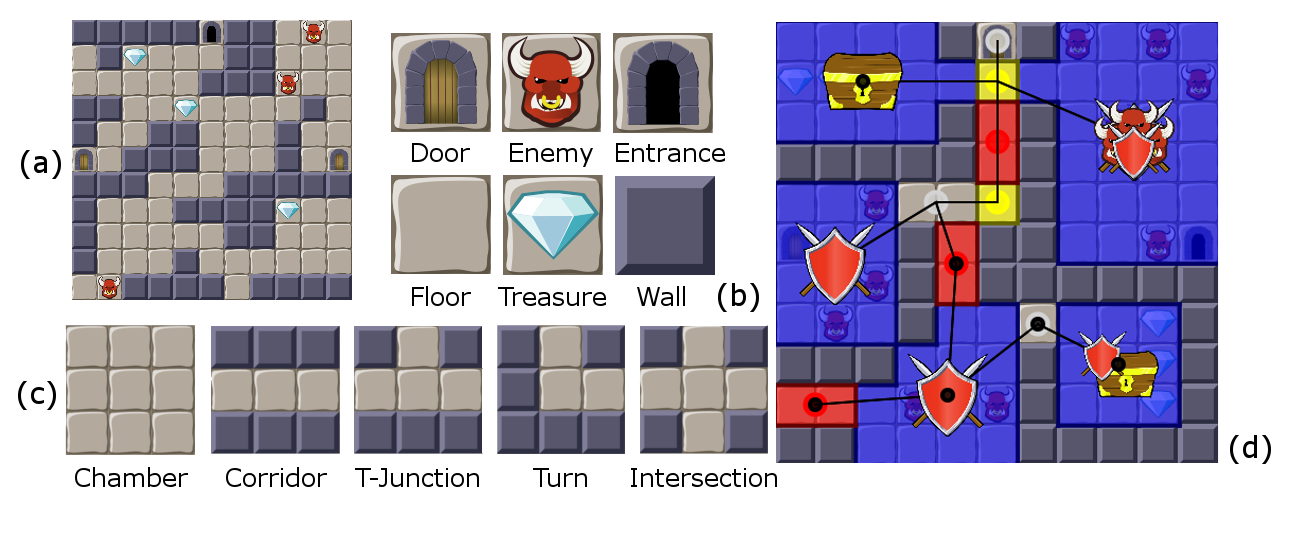
\includegraphics[width=\textwidth]{fig3.png}
\caption{A sample room in EDD (a) compose by tiles (b), spatial patterns (c) and meso-patterns (d). Detailed descriptions for these components can be found in~\protect\citepfifth{p5Baldwin2017a}.} \label{p5fig3}
\end{figure}

\begin{figure}
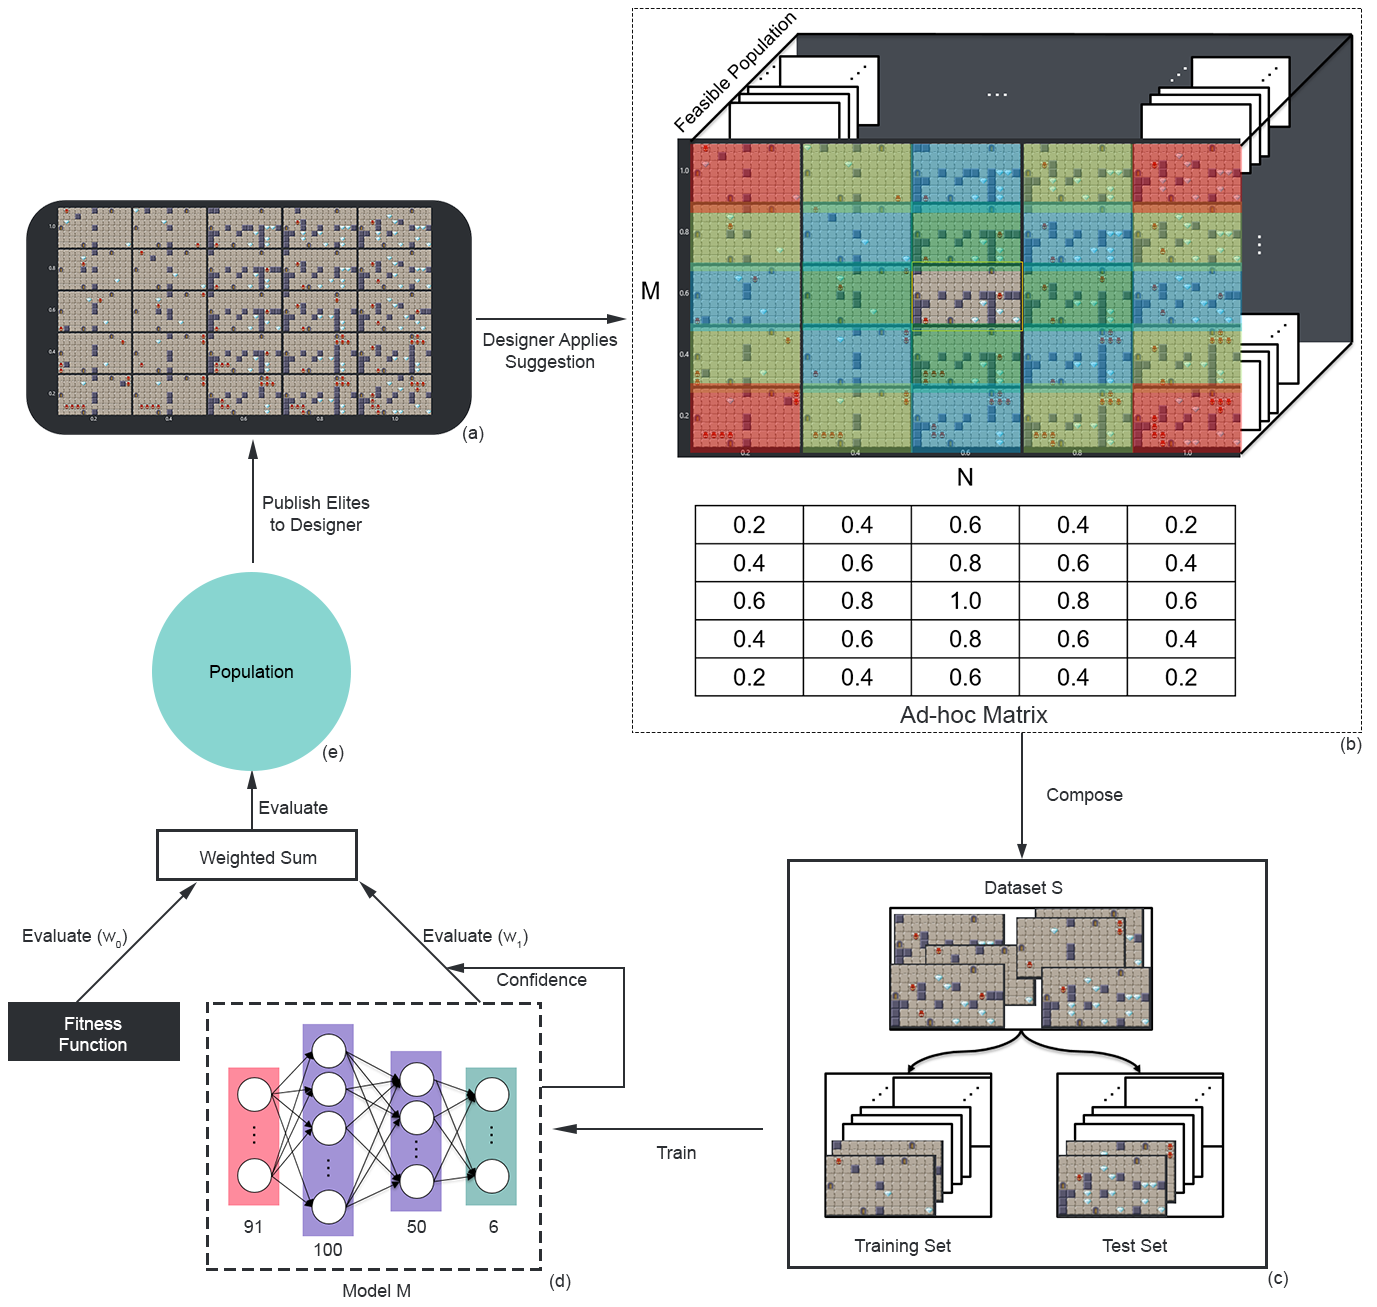
\includegraphics[width=\textwidth]{fig4.png}
\caption{Overview of the Designer Preference Model integrated into the fitness function of EDD. Elites are published and shown to the designer in a grid fashion (a), and once the designer chooses and applies one of the suggestions, an ad-hoc matrix is created based on the position of the selected suggestion to estimate the preference of suggestions (b). The ad-hoc matrix is then applied to all the elites in the grid, and the feasible populations within the EA cells to compose a general dataset $S$ with rooms labeled by the estimated preference. The composed dataset $S$ is then subdivided into a training set (90\%) and test set (10\%), both with the same label distribution (c). The dataset is used to train a model $M$, which is a relatively small neural network, for 20 epochs (d). The  model is then used to evaluate the population of the EA together with the current fitness function in a weighted sum, with the weight of the model $M$ conditioned by the confidence of the network (e).} \label{p5fig4}
\end{figure}

\subsubsection{Model Update and Usage}
The proposed model is a relatively small neural network $M$ with as many input neurons as the number of tiles composing each room, two hidden layers (100 and 50 neurons respectively), and six output neurons, one per each discrete preference value assigned to the individuals by the designer. When the designer starts EDD, the neural network is created with random initialization and without any prior training (i.e. cold start). While the designer creates and modifies rooms, on the background, the EA produces and presents individuals to the designer using the MAP-Elite’s cells (Figure \ref{p5fig2}), while it adapts to the designer’s design. Following a proactive learning approach \citepfifth{p5donmez2008proactive}, anytime the designer chooses one suggestion to replace her current design, a training session is requested for a model $M$ with a dataset $S$ created with the current cells and their populations based on the designer’s chosen suggestion. The loop, depicted in figure \ref{p5fig4}, can be described in the following two steps:

\paragraph{Dataset creation:}

The designer chooses a suggestion to replace her current design, which in turn, requests a training session using all the current individuals (i.e. the elites and the rest of the feasible populations) to create a new dataset to train the model closer to the “actual” preference of the designer. As shown in figure \ref{p5fig4}.b, an ad-hoc matrix is created, based on the position of the applied suggestion, to calculate the estimated preference, starting with the applied suggestion (1.0 preference value), and reducing the preference value by 0.2 per each step that was taken away from the applied suggestion in the matrix until a minimum of 0.0. %Once the ad-hoc matrix is created, all the individuals are given an estimated preference value based on their grid position and are used to compose a general dataset $S$. 

Once all the individuals are given an estimated preference value based on their grid position by the ad-hoc matrix, they are all used to compose a general dataset $S$ where each individual is transformed to match the network input. Finally, we divide the set into a training set (90\%) and test set (10\%) with the same label distribution. Through this process, we end up having a maximum of $M \times N \times feasible_{population}$ tuples, which relates to the granularity of each presented dimension times the maximum amount of feasible individuals per cell.

\paragraph{Training and usage:}

The model is then trained for a limited set of epochs (i.e. 20 epochs) and later incorporated into the evolutionary loop to further evaluate individuals. As mentioned above, the model tries to slowly fit towards the designer’s preference, and as it becomes more confident in predictions, the more weight $W_{1}$ it has in the final fitness of an individual. Confidence is calculated based on the output of the softmax layer, which %squashes 
limits the output of all the neurons into the range 0 to 1, as the sum of all the neurons' output must be 1.0. This characteristic of the softmax layer enables us to interpret the results as the probabilities for each of the classes. For instance, if the network predicts that an individual is going to be preferred to the designer with a 1.0 preference with a probability of 0.9, it means that the remaining 0.1 is distributed among the other output classes, and as a consequence, the network has high confidence. The resulting weights (Eq. \ref{p5eq:weights}) and weighted sum (Eq. \ref{p5eq:weightedSum}) to evaluate each of the individuals in the EA were the following:


% \begin{equation} \label{p5eq:weights}
% \begin{align}
% &w_{1}=\min(M_{conf}*M_{TestAcc}, 0.5),\\
% &w_{0} = 1.0 - w_{1}            
% \end{align}
% \end{equation}

\begin{equation} \label{p5eq:weights}
\begin{split}
 w_{1}={}&\min(M_{conf} \cdot M_{TestAcc}, 0.5),\\
w_{0} ={}& 1.0 - w_{1}   
\end{split}
\end{equation}

% \begin{align} \label{p5eq:weights}
%     w_{1}={}&\min(M_{conf} \cdot M_{TestAcc}, 0.5),\\
%     w_{0} ={}& 1.0 - w_{1}   
% \end{align}

\begin{equation} \label{p5eq:weightedSum}
weightedSum = (w_{0} \cdot objective) + (w_{1} \cdot predicted_{pref})
\end{equation}

Finally, the loop continues and the model awaits for the next training session that will be triggered the next time that the user applies a suggestion. In the meantime, the trained model is used as part of the combined individual evaluation process.
% \subsection{Concepts and Definitions}

%This paper presents an approach and fundamental steps towards the implementation of designer personas: an analysis of designer style clustering to isolate archetypical paths that can be later be used to build ML surrogate models of archetypal designers. Such models would adapt to the dynamic designer during the mixed-initiative creative process by being placed in the solution space, allowing the designer to traverse such space of models as she drifts through the many dimensions of her creative process.

% design archetypes 

Our work draws from ideas, concepts, and definitions introduced by Liapis et al., such as the core designer model loop when using CAD tools, what can be modeled: preferences, style, goals, processes, and their definition, and particularly, the use of designer modeling as an individual or collective model~\citeptenth{p10Liapis2013-designerModel}. We support our approach on the idea of style as a particular type of designer's preference, and that a collective model can be used to form a stable and static design space, which after being interacted with by designers, can be adapted towards them.

% and the idea of style as a particular type of designer's preference.

%. Moreover, Liapis et al. discuss the modeling of style as a type of preference, where each individual designer has peculiarities and characteristics that makes their style recognizable. While we agree with this vision, we 

%Our work draws from many of the ideas and concepts introduced by Liapis et al.~\citeptenth{p10Liapis2013-designerModel}, in relation to style, goals, preferences and design processes of designers. Nevertheless, given the interdisciplinary scope of this system, and the multiple concepts discussed throughout the paper, it is essential to have operational definitions on the different terms used.

%Thus, in this paper, the shared goal is set and defined by the designer with her design, and as she develops, adapts, and changes, the system seeks to adjust its goals to support the designer's work. Furthermore, the aim of this paper is to propose a system that is able to identify the designer's current goal and style to adapt further the system's goals to provide a personalized experience.

\subsubsection{Design Style} \label{sec:designStyle}

%Every designer has a different style when creating content, especially levels, where one might 

% One idea is to train a supervised learning model on traces of other collaborative creation session and try to predict the next step the human would take in the design process. The main problem with this is that people are different, and different creators will want to take different design actions in the same state;

% One way of overcoming this problem could be to change the level of abstraction at which design actions are modeled and predicted. Instead of predicting individual edits, one could identify different styles or phases of the artifact being created, and model how a designer moves from one to another. To put this concretely in the context of designing rooms for a Zelda-like dungeon crawler~\citeptenth{p10tloz}, one could classify room styles depending on whether they were enemy onslaughts, complex wall mazes, treasure puzzles, and so on. One could then train models to recognize which types of rooms a user creates in which order. By clustering sequences of styles or phases we could formulate designer personas as archetypical trajectories through style space, rather than as sequences of individual edits. For example, in the context of creating a dungeon crawler, some designers might start with the outer walls of the rooms and then populate it with NPCs, whereas another type of designer might first sketch the path they would like the player to take from the entrance to the exit and then add parts of the room outside the main path.

There exist many different styles when creating content, especially levels, that designers can create and adapt to accomplish their goals and the experiences they want for players. On a general level, \emph{Design Style} encompasses the creative process from conceptualization, prototyping, reflection, adaptation, especially when following different processes or constraints during collaboration. Taking a more concrete and operational level, \emph{Design Style} can be analyzed as overarching goals that different designers have when creating a dungeon. For instance, dungeons in games such as Zelda\citeptenth{p10tloz} or The Binding of Isaac\citeptenth{p10mcmillen_binding_2011}, represent a particular playing style planned by the designer. In the former, low tempo, exploring the dungeon, and secret rooms define the style of the dungeons, whereas in the latter, high tempo, optimizing time and resources, small rooms, and in general high-challenge define the dungeons. 

While interesting and relevant to understanding the designers' holistic design process and the expected player experience, \emph{Design Style} can also be discussed on an individual room basis. Rooms have their own set of characteristics and styles that can be identified and modeled to understand their design process. Some would prefer to create the room's architecture first to then create the goals within, whereas others would like to place strategic objectives around and then create the architecture around it or alternating between both. Even with such a division, how to reach those design styles is not straightforward and does not require the same strategy, which also shows the preference and style of individual designers. For instance, if the goal is to create a challenge to reach a door, the designer could create a room with a substantial number of enemies, create a concentrated high-challenge in the center of the room, or divide the room into smaller choke areas. Therefore, in this paper, we take a simplified view of \emph{Design Style} and treat it as the style designers follow to create a room, informed by the individual steps each has taken connected to their preferences and goals.

% While this is a simplified view of \emph{Design Style}, we acknowledge that this is a simplified view of \emph{Design Style}, as this could encompass 

% I take some issue with the framing of the paper as being one of modeling someone’s “design style” based only on the sequence of design actions taken as evidenced in snapshots of a design process. To be clear, I think the snapshot approach is a perfectly reasonable one.  But I worry that giving it a term as all-encompassing as “design style” is overpromising, because there is so much about someone’s approach to design that is lost in reducing it to a sequence of partial designs: moments of self-reflection, prototyping and throwing away ideas before moving to new ones, experimentation on paper away from the machine, prior exposure to design and how it informs new design choices, adherence to norms of genre. Obviously these cannot be captured through this approach, nor do they need to be for the work to be valid. Nonetheless, it seems unfair to characterize “design style” as a mere sequence of edit operations.

% I think more precise language would also make clearer what the strengths and limitations of this study are. By naming the aspects of design that are not captured, it makes clear what potential future work there is, how this approach should and should not be applied in other design tools, and the extent to which this work may be generalizable across tools and genres.

% I think this issue also comes up in cluster labeling. Some of the cluster labels refer to properties of room layout (e.g. “maze-like complex architecture”; “dense room”), some to meta-aspects of design (e.g. “high challenge, clear goal”), some to types of actions (e.g. “separating and populating chambers”, “balancing and optimizing”). It seems like it should be possible for a room to fall into two of these labeled clusters simultaneously (e.g. a maze-like room that has many enemies and a clear goal at the end of the maze), and it’s confusing that these are separate clusters. The same is true for other cluster pairs (e.g. “bordered rooms with deeper architectural development” and “dense, full-range leniency” seem like they could co-exist). It’s also not clear how these cluster labels are applied (other than a “qualitative analysis” — but was this done by the research team, or by external experts? how was this evaluated?).


% we use a simplified vision of \emph{Design Style}

% this general level is interesting to udnerstand the designer's holistic design process, there is a need to 

% analyzing the individual rooms gives a

% Every designer has a different style when creating content, especially levels, some would prefer to create the architecture of the room first to them proceed to create the goals within, whereas others would like to place strategic objectives around and then create the architecture around it or alternating between both. Even with such a division, how to reach those design styles is not straightforward and does not require the same strategy, which also shows the preference and style of individual designers. For instance, if the goal is to create challenge to reach a door, the designer could create a room with a substantial amount of enemies, or create a concentrated high-challenge in the center of the room, or divide the room into smaller choke areas.

% Going to a more general level, one could also think of the designs as overarching goals that different designers have when creating the dungeon. For instance, dungeons in games such as Zelda\citeptenth{p10tloz} or The Binding of Isaac\citeptenth{p10mcmillen_binding_2011}, represents a certain playing style planned by the designer. In the former, low tempo, exploring the dungeon, and secret rooms defines the style of the dungeons, whereas in the latter, high tempo, optimizing time and resources, small rooms, and in general high-challenge. While this general level is interesting to udnerstand the designer's holistic design process, there is a need to 

% the whole dungeon represents a certain playing style the design

% One can also think on the designs as a overaching goals that different designers would have, some would luike a high-tempo with smaller rooms and high challenge with minimal rewards while others might prefer the designer to go through more convoluted mazes with many connections to confuse the player and reward the understanding of patterns. While this view is interesting to understand the designer's holistic design process; in this paper we threat Design Style specifically as the style designers follow to create a room, informed by the individual steps each has taken.


% % I think i should discuss 

% % While very discussed, style 

% We can discuss this in both a specific and general level. For adventure and rogue-like games such as Zelda\citeptenth{p10tloz} or The Binding of Isaac\citeptenth{p10mcmillen_binding_2011}, the whole dungeon represents a certain playing style the design  %in-development

% \subsubsection{Designer's Goals}

% Usually, designers' goals are linked to the experiences they want to create for players, however, in a MI-CC tool, the goal is defined as the 

% It is identified as the 
% The designer's goal is defined as the current state of rooms and the set of interactions done in the tool or sequence of steps taken thus far, to reach such a state. Goals by the designer are linked to the addition and strategic placement of enemies and treasures, giving some goal for the player, e.g., forcing the fight with an enemy or allowing the player to avoid the conflict through side paths.



%Specifically, this definition is used as the current goal to be achieve by the designer identified as the sequence of steps taken thus far. Goals by the designer are linked to the addition and strategic placement of enemies and treasures, which gives some type of goal for the player, e.g. force the fight with an enemy or give the opportunity for the player to avoid the conflict through side paths. 

%Moreover, in EDD the designer is tasked to create a dungeon with an unlimited amount of interconnected rooms where each room can be further designed on it's own. When designing the dungeon and the rooms, the designers have the freedom to create the rooms as they want with any goal for the player. For instance, if the goal of the designer is to create a boss room, she might create a room with some narrow corridors that end up in a fight with a boss.



% \subsubsection{System Goals}

% The system goals are defined as the system's approach to support and foster the work of the designer by providing suggestions aligned with her current design or giving assistance, information, visualization, and measurements when needed. In general, when providing suggestions, the system aims at generating rooms among multiple areas of the generative space, simultaneously providing rooms adapted to the designer's goal and different from it. 




%The system's goal is to support the work of the designer by providing assistance, information, and measurement when needed. The system's main feature is the provided suggestions by means of the Interactive Constrained MAP-Elites~\citeptenth{p10Alvarez2020-ICMAPE}. These suggestions adapts to the current room's design by automatically modifying the fitness function in favor of the new features of the room such as enemy and treasure ratios or the balance between corridors and open chambers. Through this suggestions, the goal is to provide possible designs in the generative space for the designer while fostering her creativity by presenting suggestions that might not have been considered by her.




% \subsubsection{Shared Goals}

% The shared goals between the system and the designer are defined as the goals the designer has when creating the dungeon and the individual rooms. Thus, in this paper, the shared goal is set and defined by the designer with her design, and as she develops, adapts, and changes, the system seeks to adjust its goals to support the designer's work. Furthermore, the aim of this paper is to propose a system that is able to identify the designer's current goal and style to adapt further the system's goals to provide a personalized experience.




% \subsubsection{Design Archetypes}
%   %in-development
% Design archetypes or archetypical designer paths are used to describe and represent design processes' paths taken by designers when creating levels 
% This is akin to player archetypes~\citeptenth{p10bartle1996-taxonomy} that partition players into descriptive categories by analyzing their in-game behavior and reactions, design archetypes or archetypical designer paths are used to describe and represent 

% analyzes the behavior of players  partition players into descriptive categories 
\subsection{Designer Personas} \label{p6section:results}

%We  trained  3  models  for  each  representation  and  problem configuration. To analyze these models, we collected 40 generated levels for each model.  To generate the levels, 40 different random level layouts were generated, the models were then tasked with modifying these random layouts into good levels.   We  analyzed  the  final  modified  levels  using  different change percentages, ranging from0%to100%, where thepercentage represents the fraction of tiles the agent is allowedto change during inference

%To understand the typical progress of designers and validate the clustering, we visualize how typical design sessions traverse the various clusters. These trajectories  are  then  clustered  to  find  a  small  handful of designer personas.

\begin{figure*}[t]
    \centering
     \subfloat[\textsc{Architectural-focus}\label{p6subfig-1:dummy}]{%
       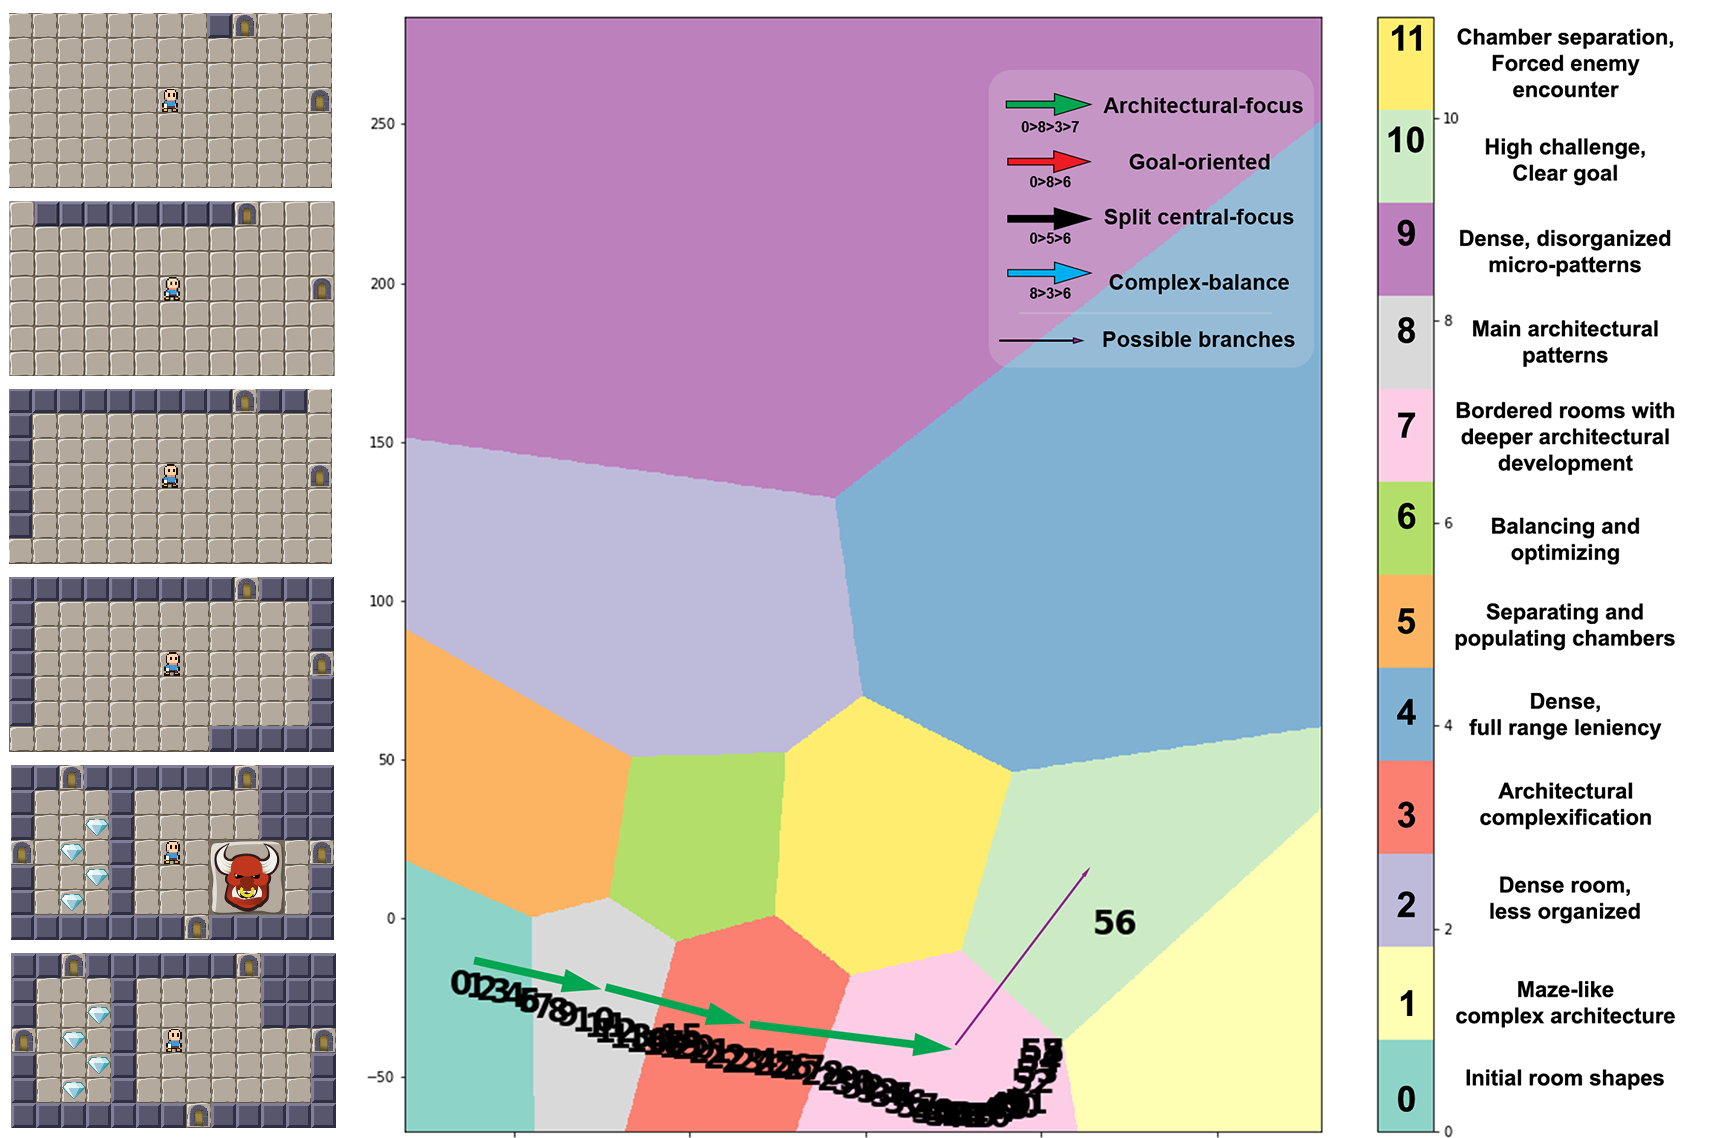
\includegraphics[width=0.45\textwidth]{figures/1.png}
     }
     \hfill
     \subfloat[\textsc{Goal-oriented}\label{p6subfig-2:dummy}]{%
       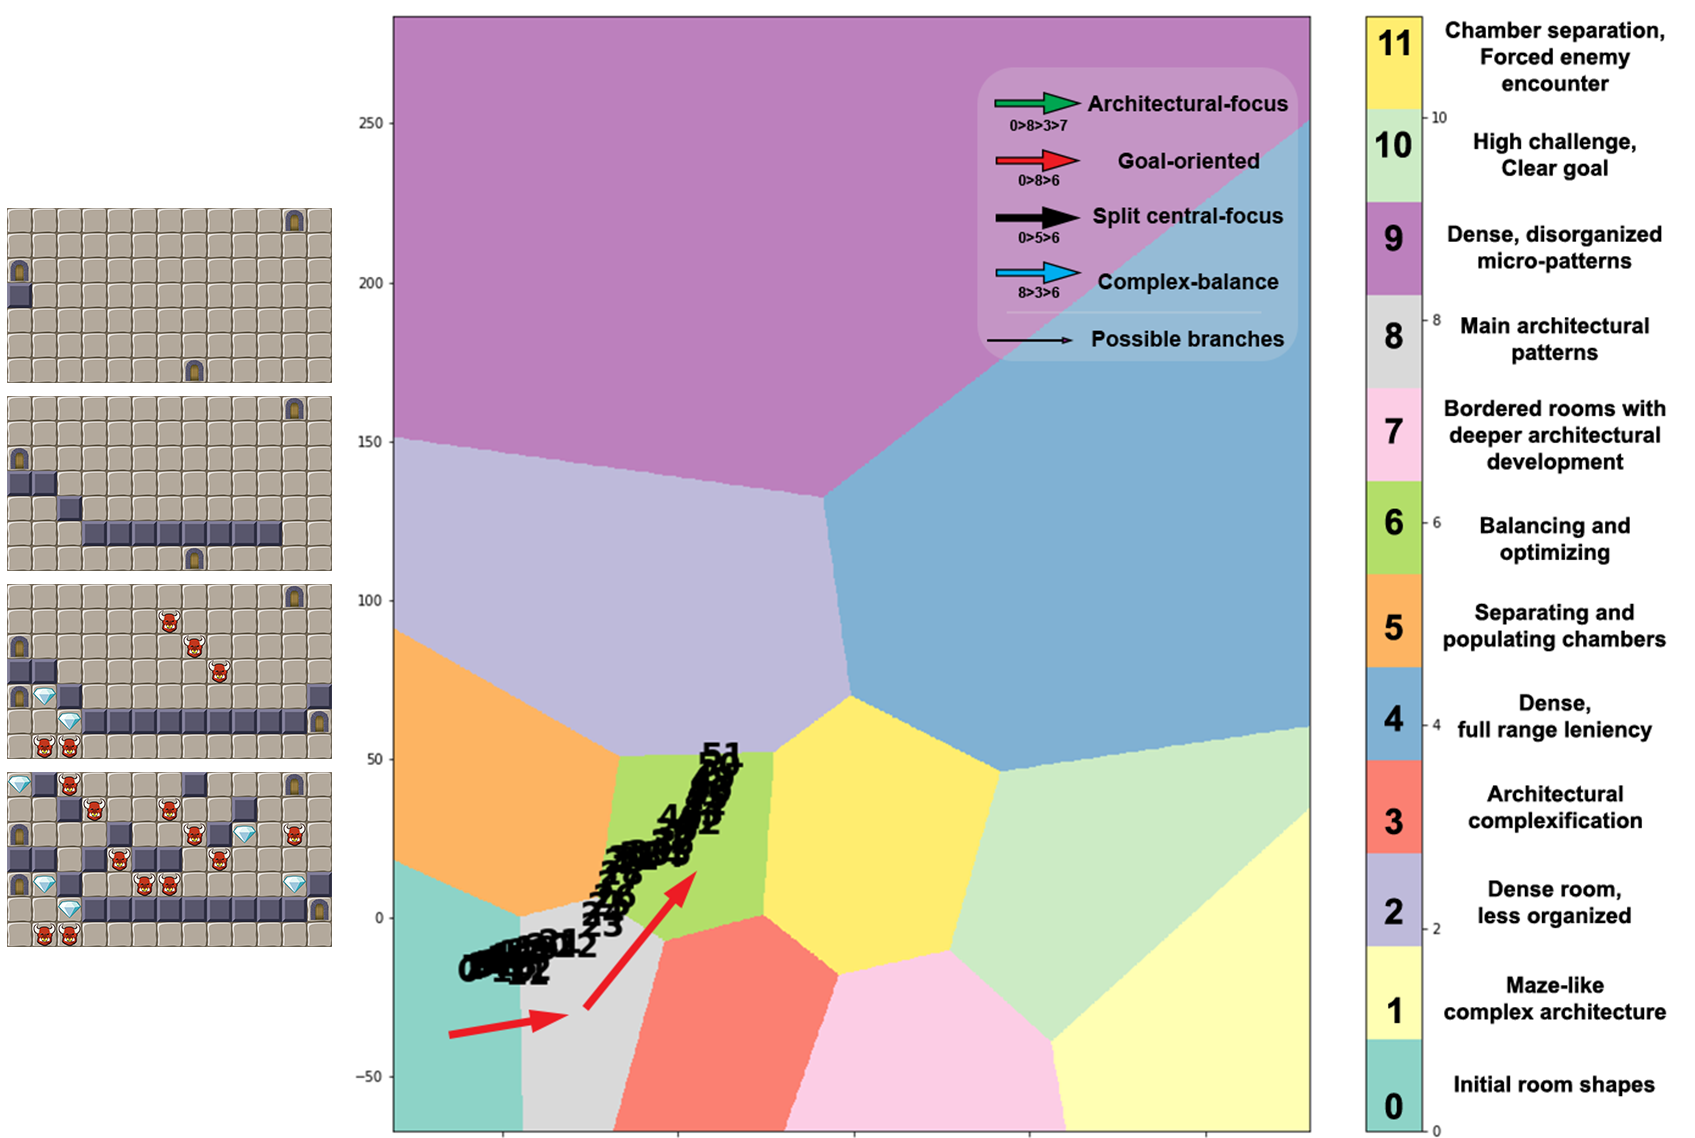
\includegraphics[width=0.45\textwidth]{figures/2.png}
     }\hfill
    %  \medskip
     \subfloat[\textsc{Split central-focus}\label{p6subfig-3:dummy}]{%
       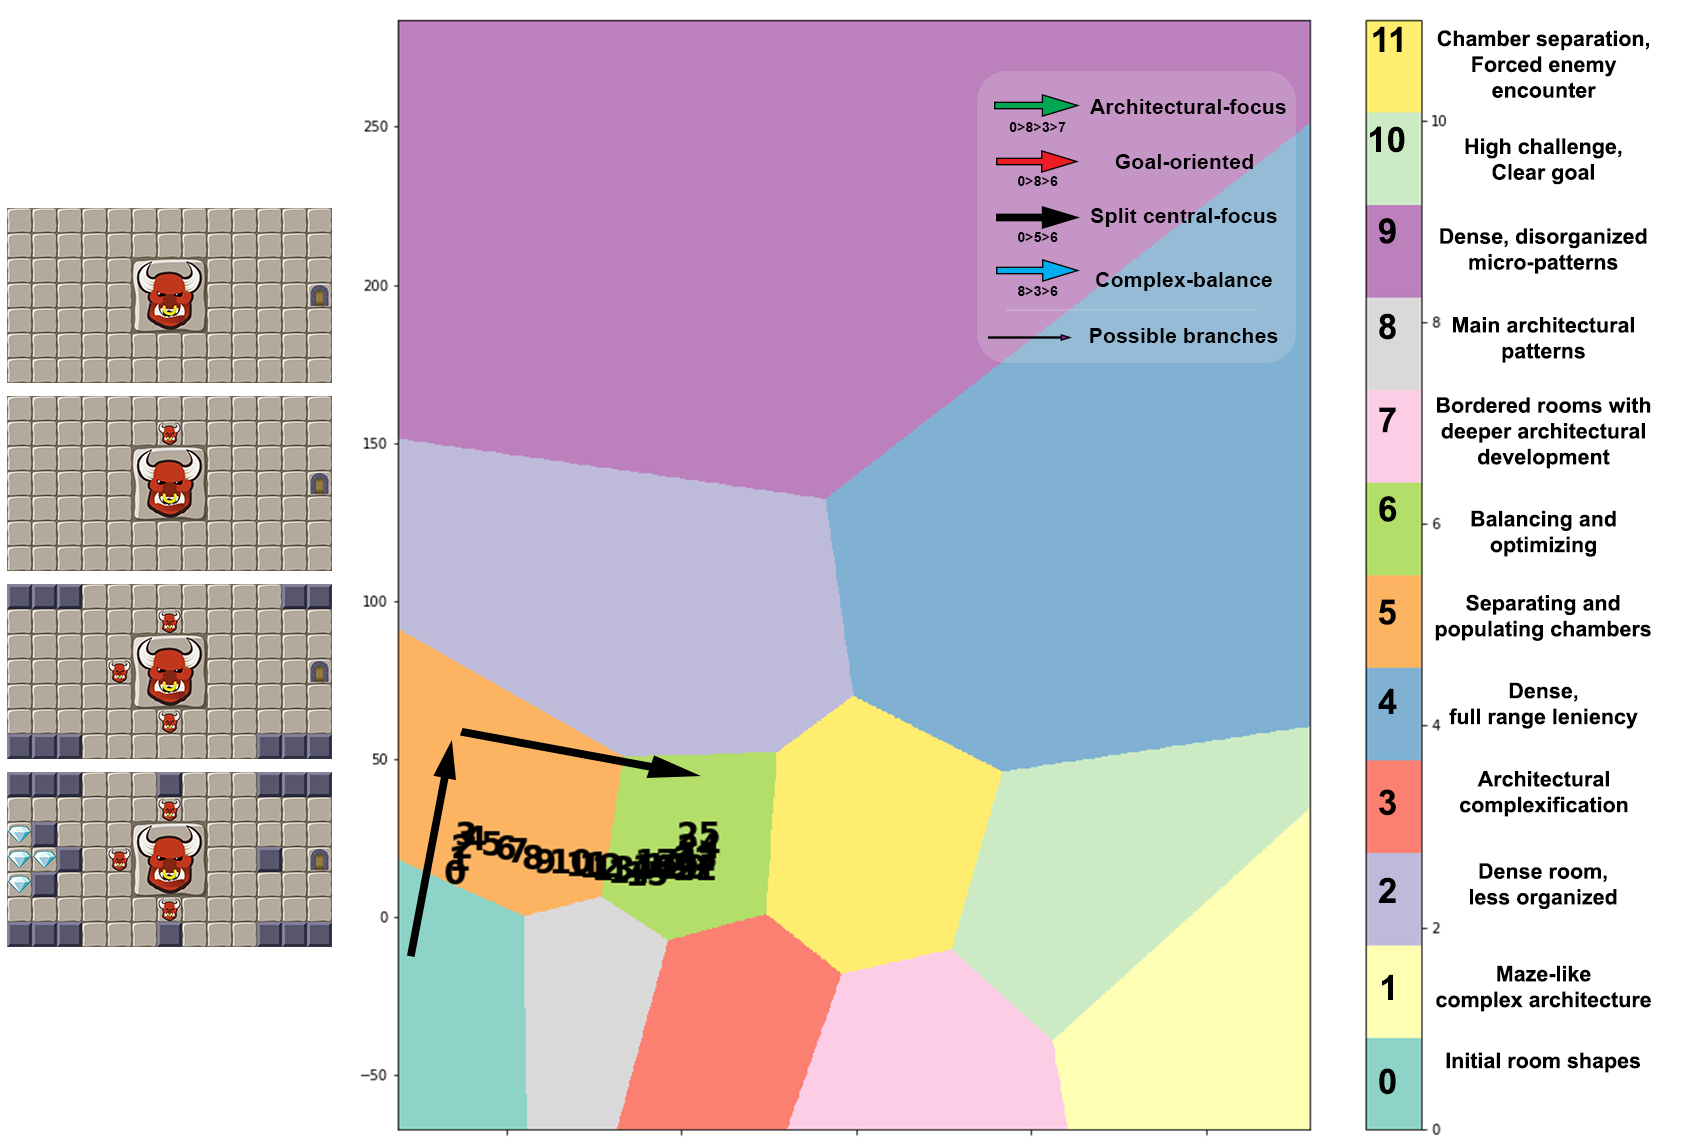
\includegraphics[width=0.45\textwidth]{figures/3.png}
     }
     \hfill
     \subfloat[\textsc{Complex-balance}\label{p6subfig-4:dummy}]{%
       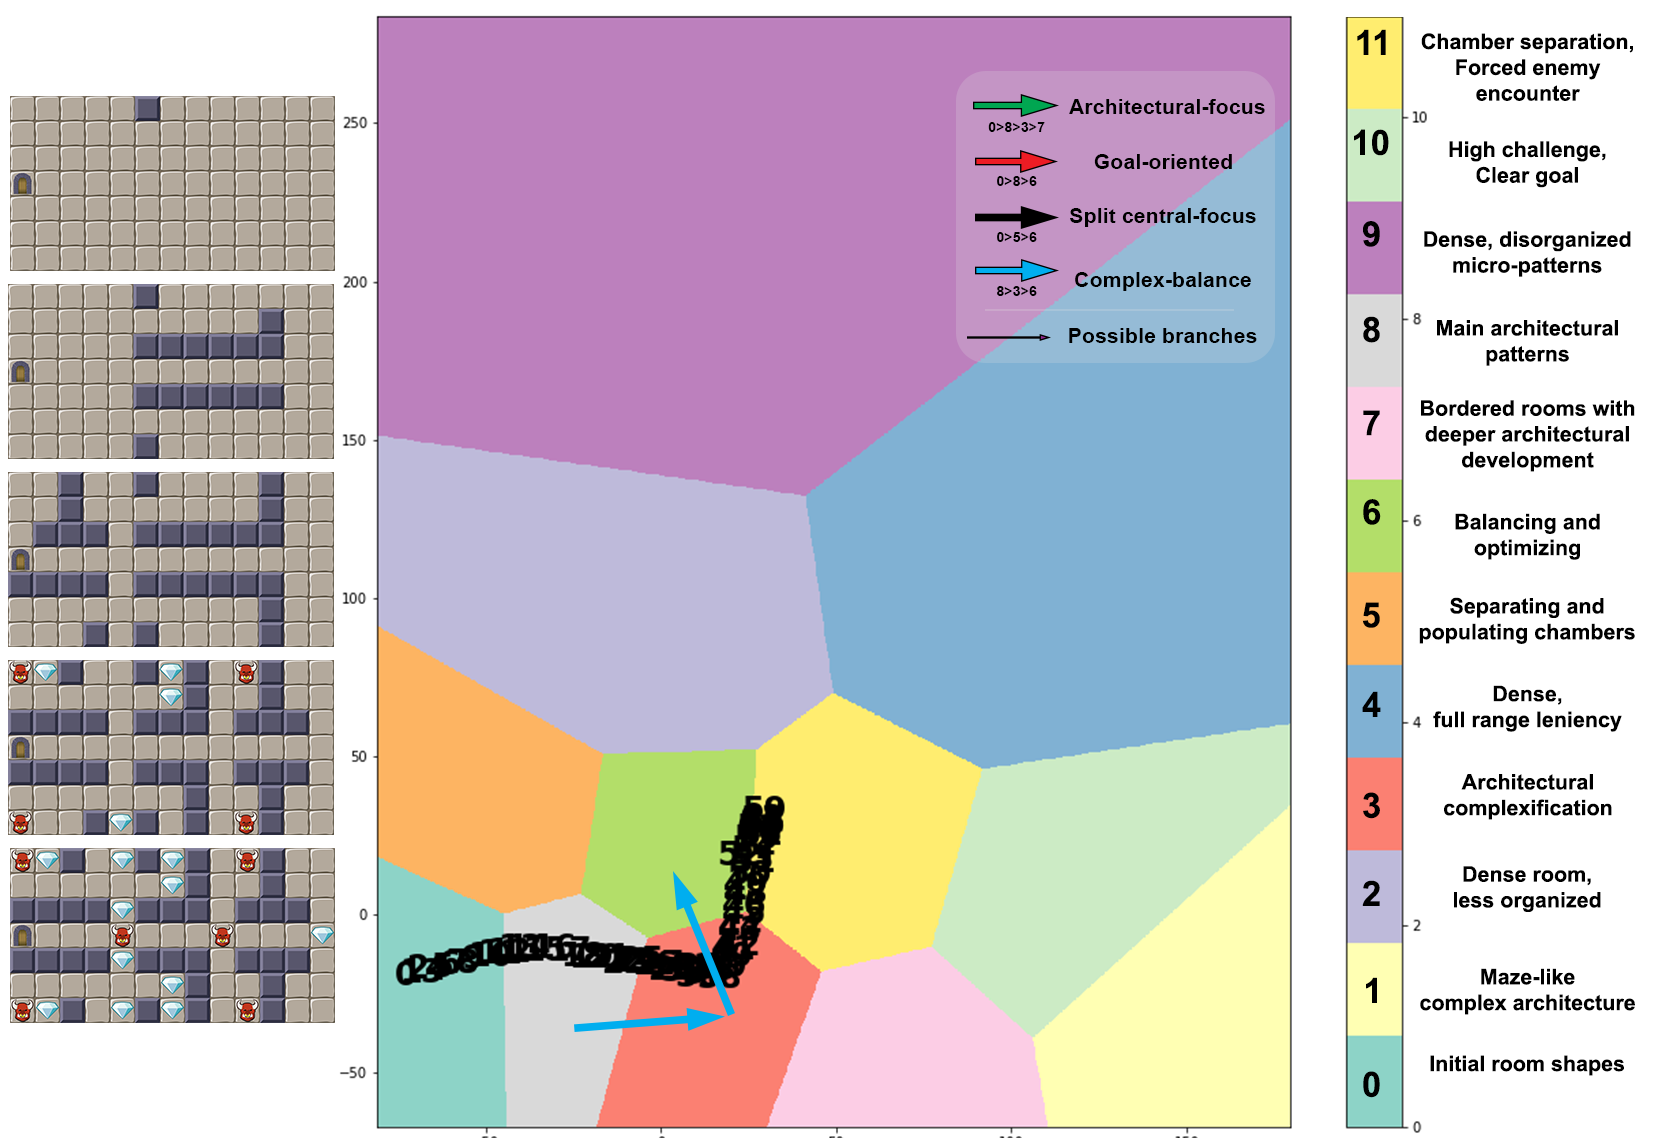
\includegraphics[width=0.45\textwidth]{figures/4.png}
     }
    
    \caption{Examples of each of the archetypical paths from one of the frequent sequences used to create the clusters. To the left of each subfigure, we present each key step in the trajectory i.e. when the design entered a new cluster. (a) presents the \textsc{Architectural-focus} archetypical path where the focus is firstly on creating the structural design of the rooms; the design process jumps back and forth suddenly to cluster 10 (one of the possible branches) due to the designer adding a boss, and removing it immediately. (b) presents the \textsc{Goal-oriented} archetypical path where the design focus on a minimal structure complexity and mix between adding structural changes and enemies/treasures. (c) shows the \textsc{Split central-focus} archetypical path where, intentionally, the designer creates a center obstacle with a boss and build around it. Finally, (d) presents the \textsc{Complex-balance} archetypical path; the design focuses on building complex, uncommon structures first and then add some goal to it with enemies and treasures, taking advantage of the spaces.}
    \label{p6fig:archetypical-examples}
\end{figure*}


Once we created, evaluated, and labeled the clusters, we were able to cluster and visualize the paths of a typical design session. Figure \ref{p6fig:paths-designers} presents an example of the design sessions, where we cluster each step of the design. This sequential process revealed that there is an interesting continuity between clusters, even capturing when a designer probably applied one of the procedural suggestions due to bigger steps in the design style clusters. Further, through this process, we could understand the progress of designers in their design process and represent their trajectory in relation to the traversed clusters rather than individual editions.

\subsubsection{Unique Trajectories}

Using the clusters in Figure \ref{p6fig:all-clusters}, we clustered the design session of all the $180$ designs and collected the unique trajectories that arose from traversing the various clusters. These unique trajectories varied in the starting point, length, and end-point, however, when analyzing the trajectories we identified common patterns among them. They had a similar shape as the following $Unique=$\{0\textgreater8\textgreater4\textgreater7\textgreater10\}, where the first and last element of the sequence are respectively, the starting- and end-points, with all the unique intermediate steps in between.

To gather the common patterns from the trajectories, we applied the Generalized Sequential Pattern (GSP) algorithm, which locates frequent subsequences in the analyzed trajectories. For instance, given three trajectories (a) \{5\textgreater1\textgreater3\textgreater11\textgreater9\}, (b) \{5\textgreater1\textgreater3\textgreater11\textgreater4\, and (c) \{0\textgreater1\textgreater3\textgreater11\}, none of these is a perfect match in its entirety, but GSP can spot that subsequences \{1\textgreater3\textgreater11\}, \{1\textgreater3\}, \{3\textgreater11\}, among others, appear with frequency $= 3$.

%(2) obtain only 1 pattern ($\{5>1>3>11\}$) with frequency=2, if searching from starting points. Finally, using GSP, we find $\{5>1>3>11\}$, $\{1>3>11\}$, $\{1>3\}$, $\{3>11\}$

%We collected these unique trajectories, and 
Furthermore, after doing a preliminary analysis, we identified some steps that we classified as ``border designs'': steps that are borderline between two clusters. These \textit{border designs} disrupted the sequence pattern mining by creating noise in the unique trajectories, specifically when these \textit{border designs} entered a different cluster for just a few steps. %we categorize them as when these "unique" noisy steps were brief.
Therefore, we filtered them out by applying a threshold $\theta = 3$, so that all subsequences inside one cluster with less than $\theta$ steps are removed from the main sequence. I.e, the sample trajectory \{0\textgreater0\textgreater0\textgreater0\textgreater8\textgreater8\textgreater8\textgreater6\textgreater8\} turns into \{0\textgreater8\} instead of \{0\textgreater8\textgreater6\textgreater8\}. Through this, we were able to reduce the noise and the search space, obtaining more meaningful and frequent patterns.

\subsubsection{Archetypical Paths through Style Space}

%Figure \ref{p6fig:finalPaths} shows the archetypical paths taken by designers when creating rooms. Represented as arrows to denote direction, 

%From all the collected unique trajectories, we identified 4 main archetypical paths, which are the ones taken most frequently by designers either as their full path or as the initial path. In Figure \ref{p6fig:finalPaths}, it is shown the archetypical paths, represented as thicker arrows to denote direction, that represent the taken by designers when creating rooms. 

In Figure \ref{p6fig:finalPaths}, we present the archetypical paths, represented as thicker arrows to denote direction, which show the most frequent paths taken by designers either through their whole design process or as the initial meaningful steps. From all the collected unique trajectories, we have identified 4 main archetypical paths, labelled, \textsc{Architectural-focus}, \textsc{Goal-oriented}, \textsc{Split central-focus}, and \textsc{Complex-balance}. In addition, we have numbered each cluster for easier visualization and referencing. 

Moreover, in the figure, it can also be observed thinner purple arrows pointing to different clusters from several of the clusters that are part of the main paths. These are \textit{possible branches} presented in the unique trajectories and added based on their frequency. Through these possible branches, the design of an archetypical session, can vary and extended or deviate the final design. Each archetypical path is defined and explained as follows: 

\paragraph{Architectural-focus}The path followed by this archetype focuses first on designing the architecture of the room with walls. Through this, the design focuses on shaping the visual patterns, chambers, and corridors to give a clear space for adding goals and objectives with enemies and treasures. The sequence is denoted with a green arrow in Figure \ref{p6fig:finalPaths}, and following the sequence \{0\textgreater8\textgreater3\textgreater7\}.

\paragraph{Goal-oriented}Design processes following this archetypical path, create the rooms in a more standard way, combining simpler symmetric wall structures with distributed placement of enemies and treasures. Thus, rather than focusing extensively on an individual part of the room, the rooms have an initial structure and then they are populated with some specific goal-in-mind. The sequence is denoted with a red arrow in Figure \ref{p6fig:finalPaths}, and following the sequence \{0\textgreater8\textgreater6\}.

%Thus, rather than focusing on an individual part of the room until satisfied, the rooms have some initial structures that are populated and continue through an iterative process between these steps.% rooms go through an iterative process of adding have some initial structures that are

\paragraph{Split central-focus}This archetypical path focuses on designing rooms with obstacles placed in the center of the room in the shape of enemies, treasures, or wall structures that clearly split the room into different areas. The design process is less organized than the other archetypes since it searches to achieve the split goal with any of the available tiles. The sequence is denoted with a black arrow in Figure \ref{p6fig:finalPaths}, and following the sequence \{0\textgreater5\textgreater6\}.
%, since the middle step is cluster 5 ("Separating and populating chambers"), which relates to rooms which are expected since the cluster 5 ("Separating and populating chambers") relate to rooms that  as specific structural shapes are not necessary. 

\paragraph{Complex-balance}This archetypical path focuses on building complex symmetric shapes with a clear objective for the player and adapting the spaces with a balance of enemies and treasures. In general, the rooms created following this path are more unique and typically balanced. %   with that adapt well. The process is quite 
The sequence is denoted with a blue arrow in Figure \ref{p6fig:finalPaths}, and following the sequence \{8\textgreater3\textgreater6\}.

Furthermore, using these archetypical paths, we can then categorize certain clusters as key clusters or being more relevant than others based on their contribution to the paths, their frequency, and their usage. Most of the paths go through or end in cluster 6 (``Balancing and optimizing'') and cluster 8 (``Main architectural patterns''), which relate to rooms that have a more explicit mix between corridors and small chambers and more clear architecture. The rooms in those clusters are or shaped as end rooms, as in the case of cluster 6, or architecturally shaped to be “optimized” to a specific goal e.g. a dense bordered room. Similarly, most of the sequences start from cluster 0 ("Initial room shapes"), with $134$ out of the $180$ designs, which correlates to the type of designs encountered in that clusters. Thus, it is understandable that most of the archetypical paths pass through any of these three clusters. 

Nevertheless, it is the steps in-between what creates a clear differentiation between the archetypical paths, which is the benefit of observing the design process as a whole in the clustered room style space. For instance, in fig.~\ref{p6fig:finalPaths}, it can be observed that \textsc{Split central-focus} starts in the same cluster as three other paths, and tentatively ends in the same cluster as three other. However, the designs following \textsc{Split central-focus} are more different to the other trajectories, since it enters a cluster that is denser with several tile types in principle, and where designers seem to have a clearer goal.
% With this, we can further understand why \textsc{Split central-focus} is more different to the other trajectories, since it enters a cluster that is "less organized" in principle. 

%Furthermore, we can also observe that certain clusters are key steps for most paths because they are or a frequent starting or ending point. Most of the paths go through or end in cluster 6 ("Balancing and optimizing") and cluster 8 ("Main structural patterns"), which relate to rooms that have a more explicit mix between corridors and small chambers and a more clear structure, thus, it is understandable since the rooms in those clusters are or shaped as end rooms, as in the case of cluster 6, or structurally shaped to be “optimized” to a specific goal (E.g. dense bordered room, maze-like, more challenging, etc.). However, the distribution of endpoints is quite even, and meanwhile, cluster 6 and cluster 11 ("Chamber separation, Forced enemy encounter") are the most frequent ending points with $36$ and $25$ out of $180$ design processes, the rest of clusters are quite close.

%Similarly, most of the sequences start from cluster 0 ("Initial room shapes"), with $134$ out of the $180$ designs, which correlates to the type of designs encountered in those clusters.

Moreover, in figure~\ref{p6fig:archetypical-examples}, we present examples of each of the designer personas by visualizing the sequence of steps done in representative design sessions, showing how these paths would look like in practice. Each visualization of a designer persona has the key design steps to the left, where each image is in a sequence: the first is the first edition of the designer, the last is the final edition, and the in-between represent entering a new room style cluster. 

In (a), it is shown the \textsc{Architectural-focus}, where the designer first created the border of the room with a clear chamber division. As the designer adds and subsequently removes the boss, the design jumps to cluster 10, which is one of the possible branches, adding a high challenge. In (b), it is shown the \textsc{Goal-Oriented}, where the designer sketched the main shape of the room followed by alternating between enemies, treasures, and walls to design the goal of the player within the room. In this example, the designer ends the design close to cluster 9, with a disorganized placement of tiles and a less aesthetical room, but forming small choke areas balancing the placement of enemies and treasures.

In (c), it is shown the \textsc{Split Central-focus}, where the designer directly started by adding a boss in the center of the room and using this as a reference point, shaped the rest of the room. In (d), it is shown the \textsc{Complex-balance}, where the designer focused on creating an uncommon structure and followed by adding enemies and treasures symmetrically, with clear individual areas for the player to approach.

% It is not surprising to focus on the center as it 

Finally, further analyzing figure~\ref{p6fig:archetypical-examples}, it can also be observed an interesting dual tendency of the designers in the archetypical paths. This dual tendency is to either focus on the aesthetic configuration of the room based on what is perceived in the editor exemplified the personas: \textsc{Architectural-focus} and \textsc{Split central-focus}, and to focus on the player experience exemplified the personas: \textsc{Goal-oriented} and \textsc{Complex-balance}. Nevertheless, both are not mutually exclusive, instead this illustrates adequately the dualistic role the designer has when using the tool and designing rooms. That of creating an aesthetically pleasing object as it is seen in the editor, and that of creating an experience.% However, this is not mutually exclusive. Instead, it shows 


% Furthermore, when analyzing how the different design sequences were clustered and forming the designer personas, we observed an interesting dual tendency of the designers. This dual tendency is to either focus on the aesthetic configuration of the room based on what is perceived in the editor through the personas: \textsc{Architectural-focus} and \textsc{Split central-focus}, and to focus on the player experience through the personas: \textsc{Goal-oriendted} and \textsc{Complex-balance}. This exemplified quite good 
% dualistic role 
% When forming the designer personas, and analyzing how different design sequences


%where the designer focused on creating the shape of the room before adding any enemyfirst created the border of the room

% Finally, in Figure \ref{p6fig:archetypical-examples}, we present examples of each of the archetypical paths to show how would these paths look like in practice, further supporting our findings and path definitions. 

% The archtypical paths a dual tendency of the designers to either go for a strategy that reflects their perception of the level from the editor - like the aesthetic configurations of it, instead of the experiential ones. for example the ones that had a split central focus and a structural focus (which btw maybe i would change to architectural focus). and then there's the ones that have a focus on the player experience like the goal oriented and complex behavior ones. i think this split reflex a very nice dualistic role that the designer has in front of the editor - that of creating an aesthetically pleasing object, as they see it in the editor, and that of creating an experience.
% , and exmplified
%That build around



% Notice that not all the clusters have connectionthat based on the unique trajectories, where designers decided to move towards other areas. 

%it is shown the archetypical paths, represented as thicker arrows to denote direction, that represent the taken by designers when creating rooms. 
% moving from 6 to 11 or from 3 to 11 is a fairly frequent step, thus making it and cluster 6, key points.
% In fact, ending the design at 7 is not that common, thus, 



% the red cluster with $95$ out of the $180$, and from the purple cluster with $49$ out of the $180$, which correlates to the type of designs encountered in those clusters, mainly emptier rooms with initial sketches and shapes. 

% Most of the paths start in cluster 0 ("Initial room shapes") 

% From the figure, we can extract the following clusters as key steps for most of the patterns: "light green", "light blue", "red", and "purple". 

% It can be observed that most of the paths end or go through the "light green" and "light blue" clusters. Both relate to rooms that have a more clear structural pattern and more explicit mix between corridors and small chambers, thus, is understandable since the rooms in those clusters are or shaped as end rooms or structurally shaped to be “optimized” to a specific goal (E.g. dense bordered room, maze-like, more challenging, etc.). Quantitatively, most of the sequences end up in those clusters, $64$ out of the $180$ end in cluster 6 (light blue) and $52$ out of the $180$ end in cluster 11 (light green).


% Similarly, most of the sequences start from the red cluster with $95$ out of the $180$, and from the purple cluster with $49$ out of the $180$, which correlates to the type of designs encountered in those clusters, mainly emptier rooms with initial sketches and shapes. 


% \begin{figure*}
% \centerline{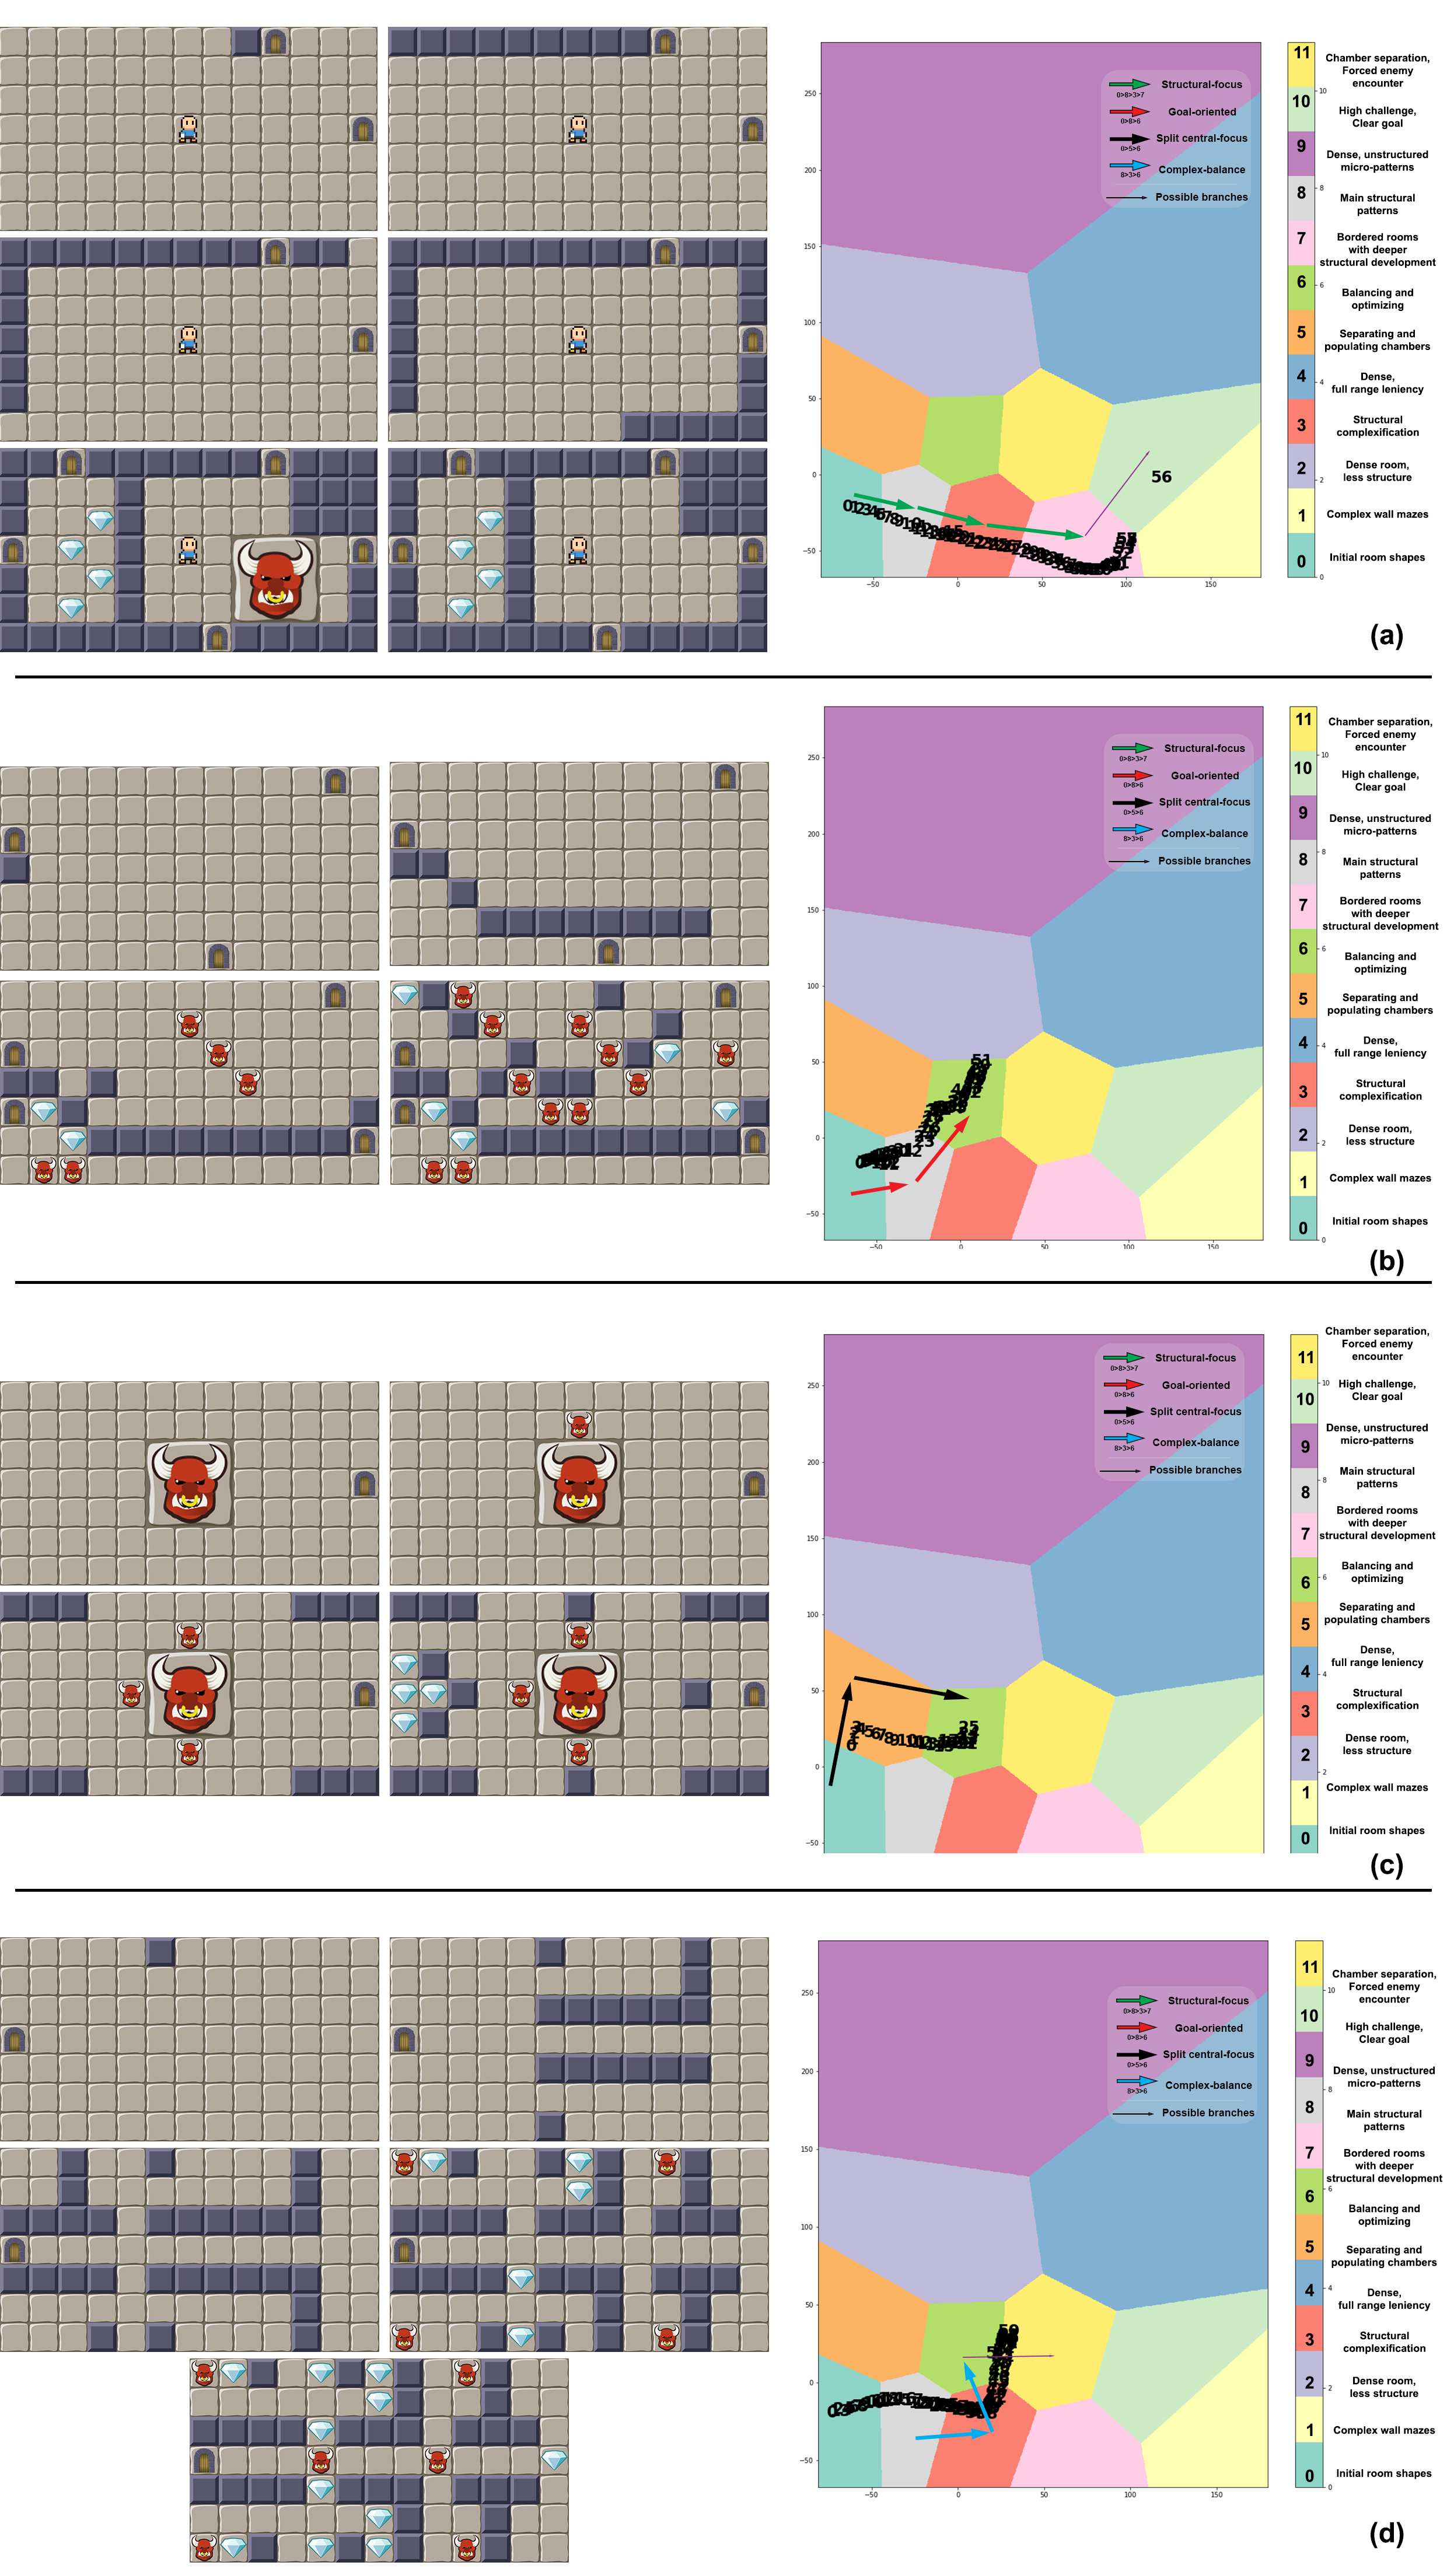
\includegraphics[width=0.7\textwidth]{figures/path-examples-2.png}}
% \caption{Examples of each of the archetypical paths from one of the frequent sequences used to create the clusters. To the left of each subfigure, we present each key step in the trajectory i.e. when the design entered a new cluster. (a) presents the \textsc{Structural focus} archetypical path where the focus is firstly on creating the structural design of the rooms; the design process jumps back and forth suddenly to cluster 10 (one of the possible branches) due to the designer adding a boss, and removing it immediately. (b) presents the \textsc{Goal-oriented} archetypical path where the design focus on a minimal structure complexity and mix between adding structural changes and enemies/treasures. (c) shows the \textsc{Split central-focus} archetypical path where intentionally, the designer creates a center obstacle with a boss and build around it. Finally, (d) presents the \textsc{Complex-balance} archetypical path; the design focuses on building complex uncommon structures first and then add some goal to it with enemies and treasures, taking advantage of the spaces.} \label{p6fig:archetypical-examples}
% \end{figure*}



% \begin{subfigure}[t]{0.33\textwidth}
%         \centering
%         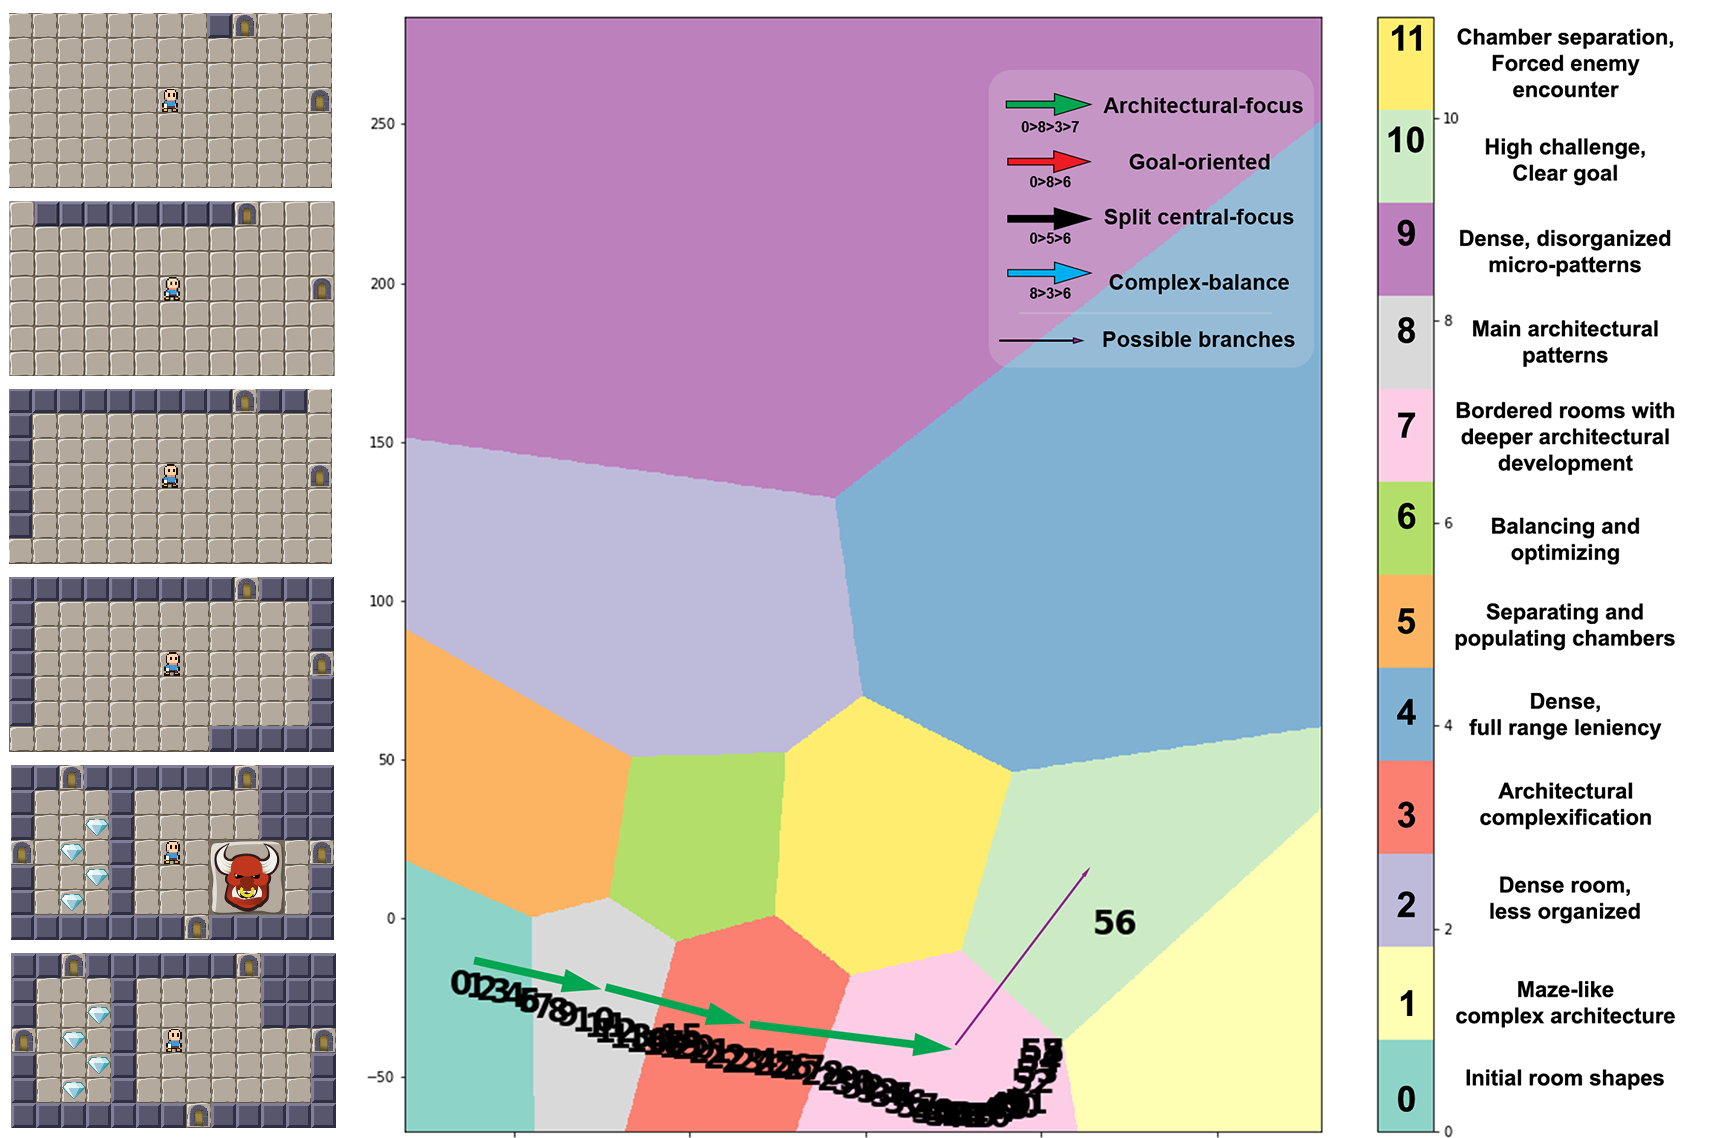
\includegraphics[width=0.95\textwidth]{figures/1.png}
%         \caption{Linearity-\#MesoPatterns}
%     \end{subfigure}%
%     \begin{subfigure}[t]{0.33\textwidth}
%         \centering
%         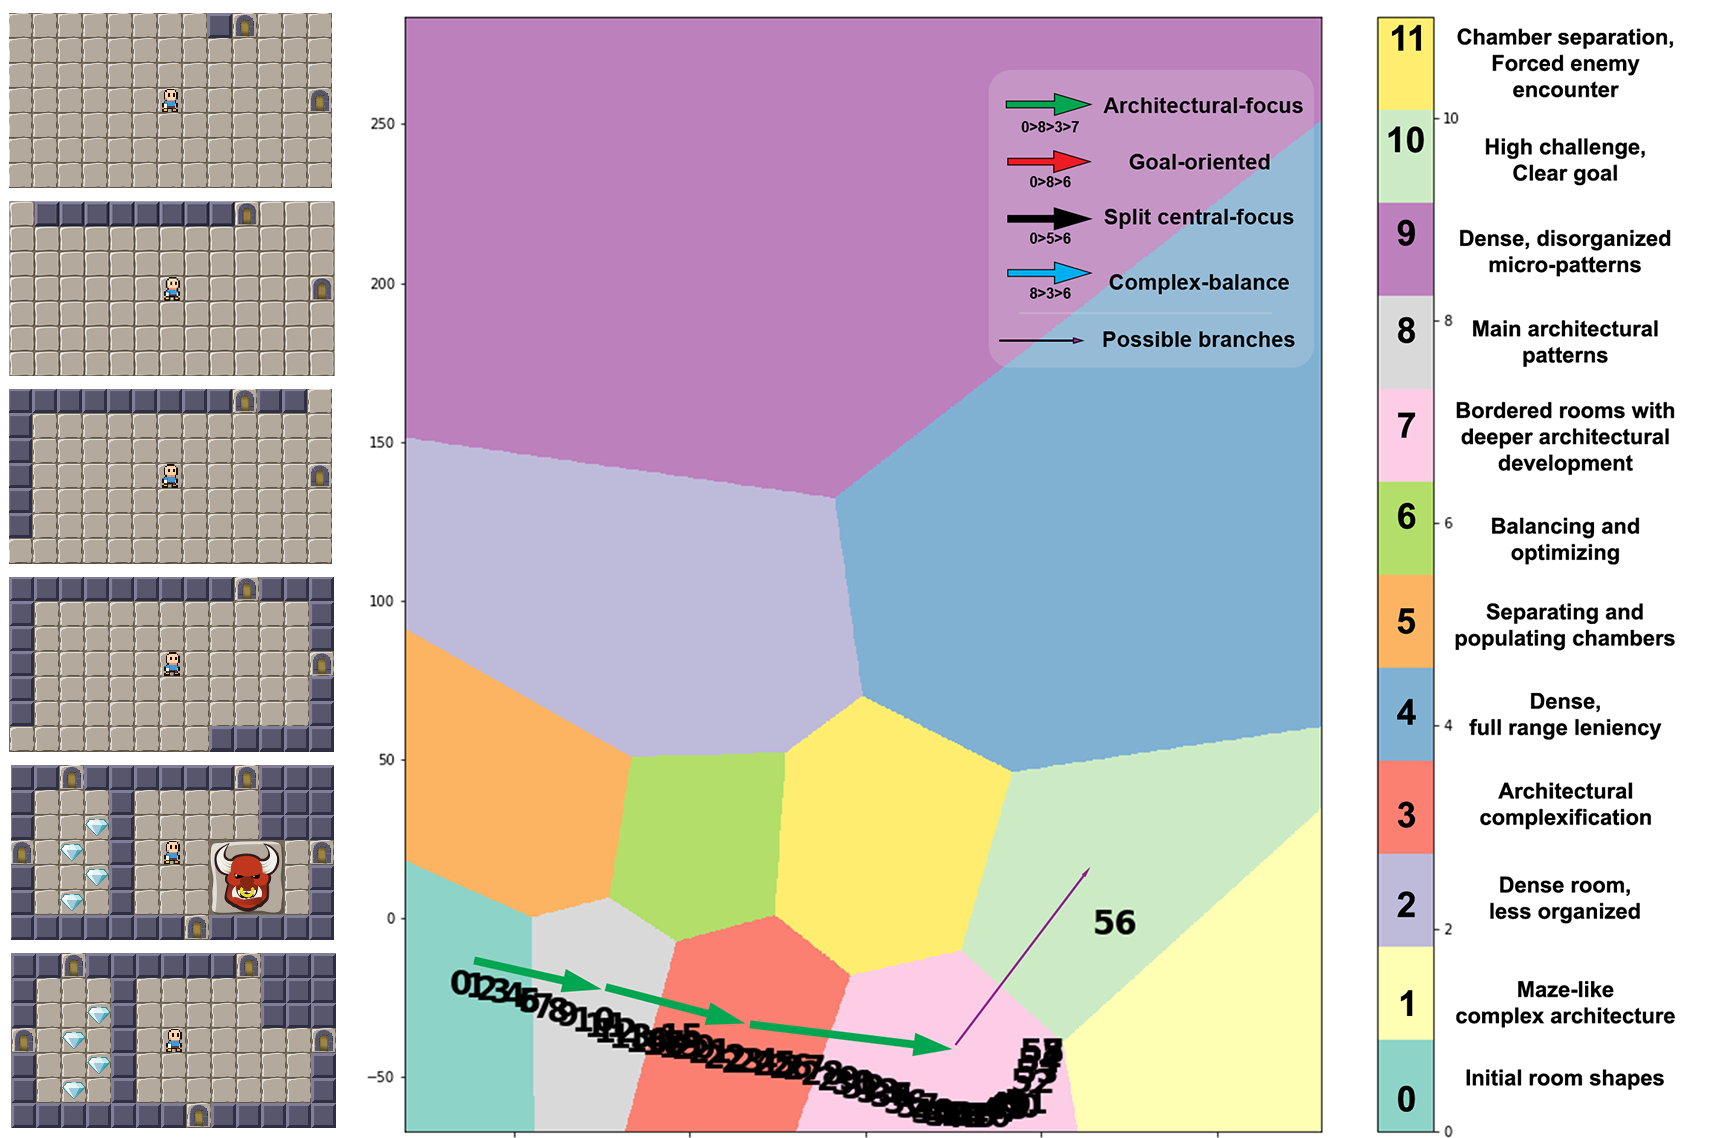
\includegraphics[width=0.95\textwidth]{figures/1.png}
%         \caption{Linearity-\#MesoPatterns}
%     \end{subfigure}%
%     \begin{subfigure}[t]{0.33\textwidth}
%         \centering
%         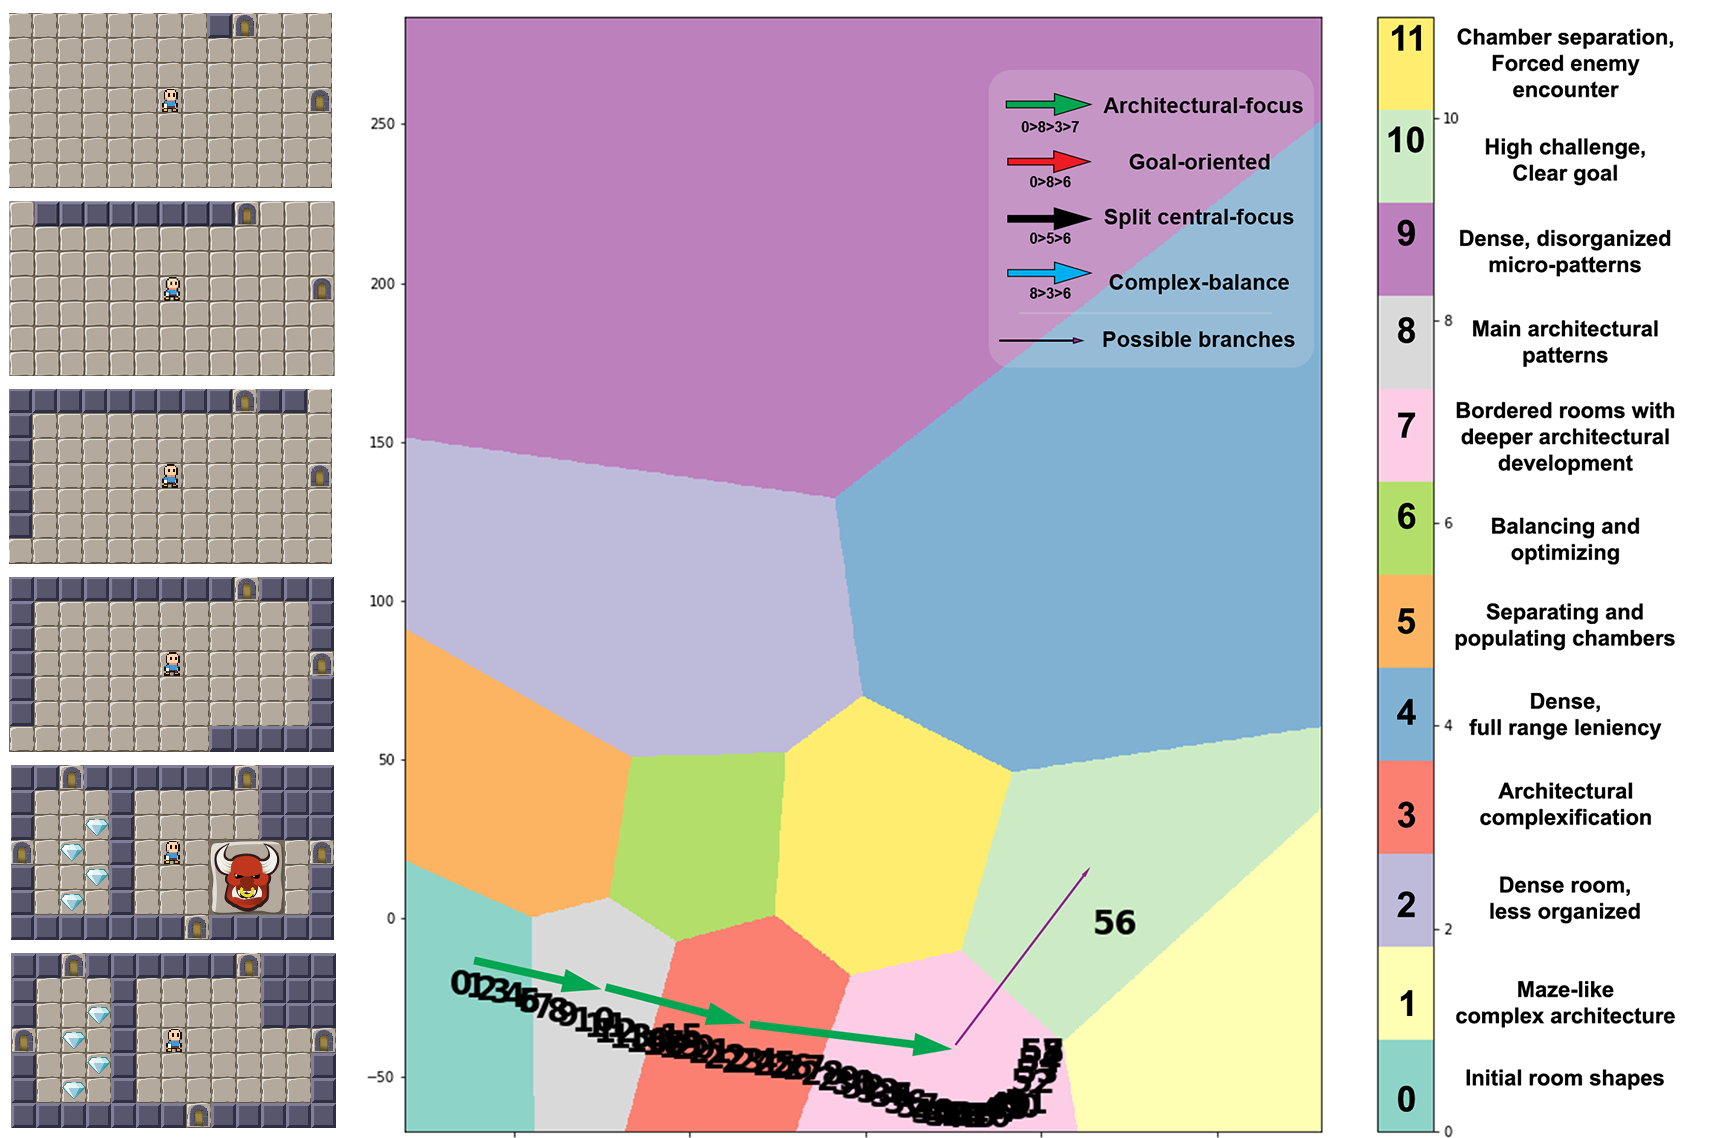
\includegraphics[width=0.95\textwidth]{figures/1.png}
%         \caption{Linearity-\#MesoPatterns}
%     \end{subfigure}%
%     \begin{subfigure}[t]{0.33\textwidth}
%         \centering
%         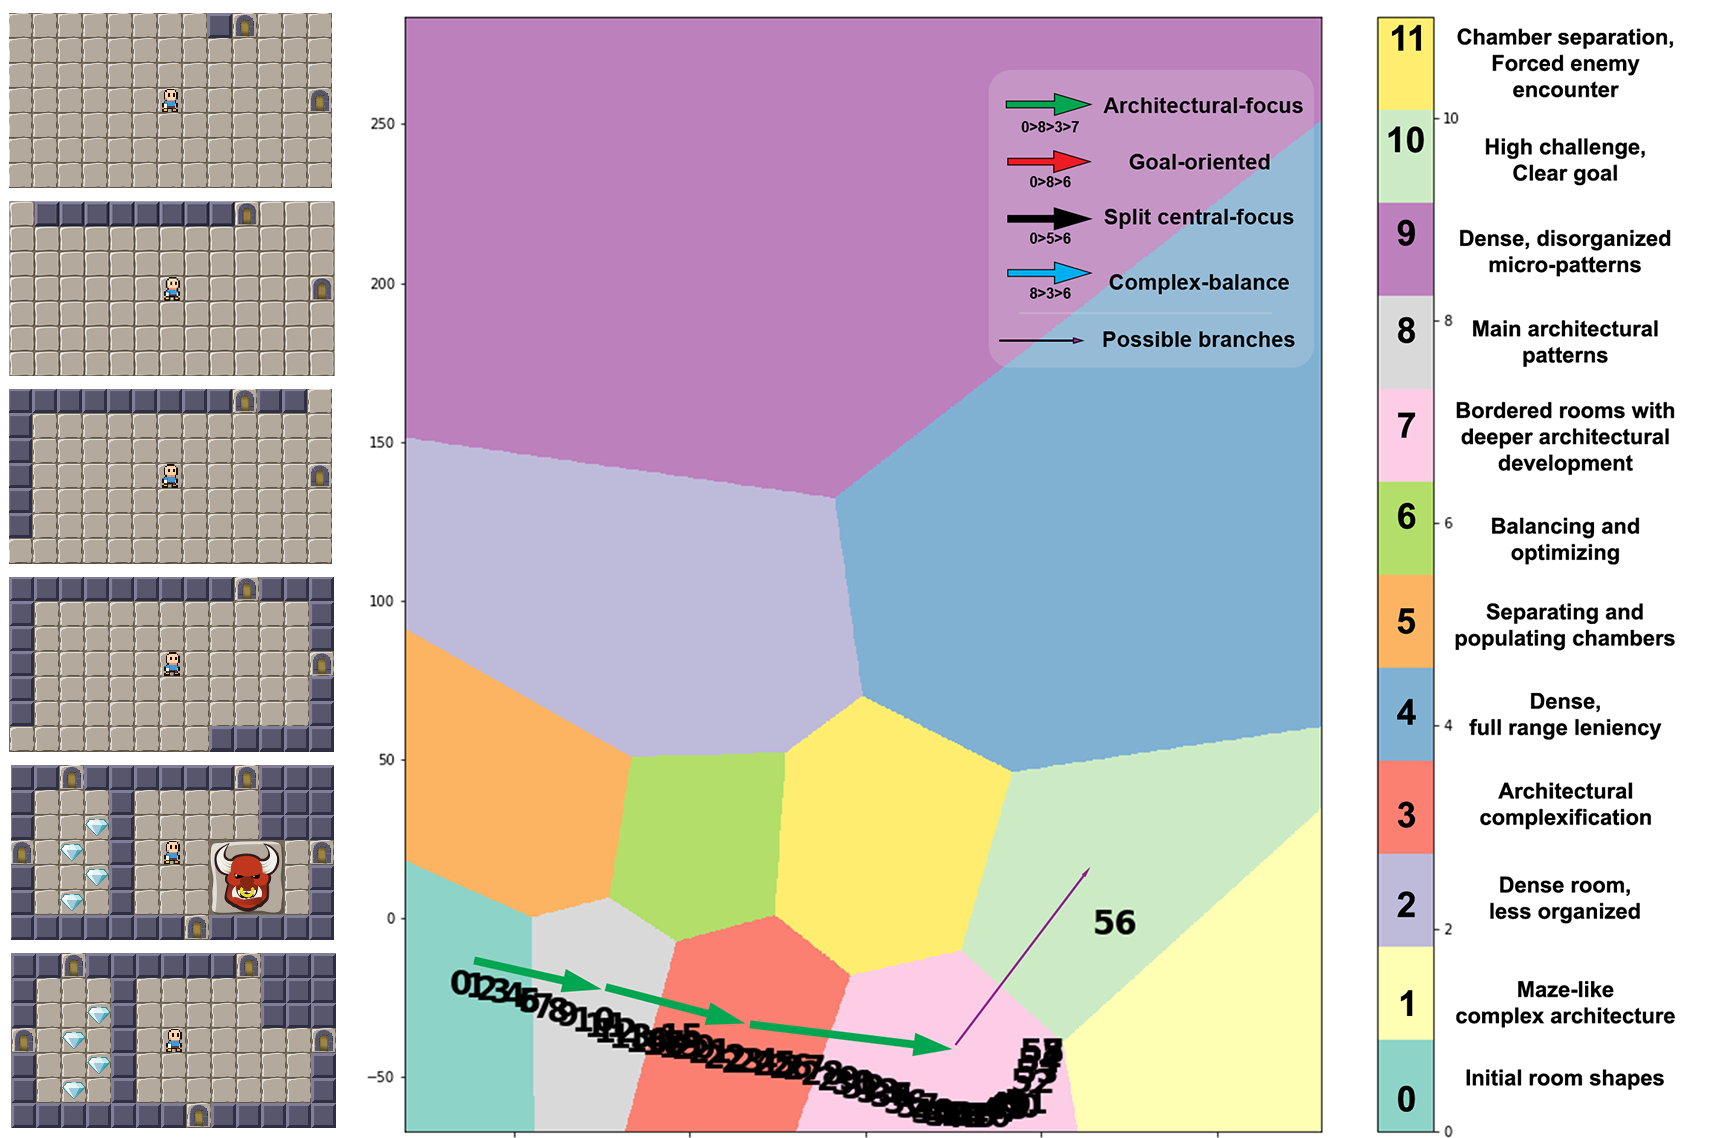
\includegraphics[width=0.95\textwidth]{figures/1.png}
%         \caption{Linearity-\#MesoPatterns}
%     \end{subfigure}%

%From the figure, it can be observed that most of the paths end or go through the "light green" and "light blue" clusters. Both relate to rooms that have a more clear structural pattern and more explicit mix between corridors and small chambers, thus, is understandable since the rooms in those clusters are or shaped as end rooms or structurally shaped to be “optimized” to a specific goal (E.g. dense bordered room, maze-like, more challenging, etc.). Further, most of the sequences end up


%Most of the rooms end there, 64 end in cluster 6 (light blue) and 52 end in cluster 11 (light green), so it makes sense that they are key steps in most of the subsequences. Further, most of the rooms start in cluster 0 (red) – 95 rooms – or in cluster 8 (purple) – 49 rooms, which make them key steps as well

%Most of the sequences with $95$ out of the $180$ starting in the red cluster, and $49$ out of the $180$ starting in the purple cluster. which correlates to the type of designs encountered in those clusters, mainly emptier rooms with initial sketches and shapes. 


%Info about the trajectories, 1) variation (length), 2) starting cluster, 3) end-point cluster.


% \begin{itemize}
%     \item[\textbf{DONE:}] Present 3 representative examples where we cluster each step of the design process. Perhaps I should create a room that would go through all the clusters?
%     \item[\textbf{DONE:}] Explain that we did this for all the 180 designs, and we collected the unique trajectories along the clusters, reducing the dimensionality of each step to each cluster.
%     \item[\textbf{DONE:}] Due to border designs (step that are in the border between 2 different clusters), we applied a threshold to reduce the noise those inputs could have when clustering the trajectories of the designer.
%     \item[\textbf{DONE:}] this data (the sequences) were then applied the GSP algorithm, a subsequence frequent pattern mining algorithm, to extract the frequent patterns in the sequences (including subsequences within the sequence).
%     \item This resulted in the following trajectories, which can also be observed in Figure X.
%     \item 
% \end{itemize}

\subsection{Conclusions}



% \begin{itemize}
%     \item Discussion on what does this archetypical design trajectories mean?
%     \item how to use them? next steps into integrating this into a system. To use this in a search-based approach as objectives for the generation to move towards the directions where (according to our archetypical design trajectories) the designers will move towards in their design process. Perhaps I could also bring the discussion from the workshop-paper for HC-AI.
%     \item discussion on creativity? is the output or the process where the actual creativity is outputted? Compare using end-design clustering to using sequences to cluster.
%     \item Discussion on how PCGRL relates to this type of work? --> Perhaps this is something for the background instead.
% \end{itemize}{}


% This paper presents a step towards designer modelling in a MI-CC environment by providing an implementation of designer personas as archetypical trajectories through style space, as a means to characterize several representative and frequent design styles together. 

%This paper presents a novel approach and meaningful steps towards designer modeling in an MI-CC environment. By providing an implementation of designer personas as archetypical trajectories through style space, we show that 

This paper presents a novel approach and meaningful steps towards designer modeling through an experiment on archetypical design trajectories analysis in an MI-CC environment. Through this, we characterize several representative design styles as designer personas. We have first run and compared several clustering setups to find the best partitioning of the design style using the edition sequences of the collected $180$ unique rooms, ending in $8196$ data points, and resulting in a set of twelve cohesive, coherent, and meaningful clusters. We have then mapped these $180$ design sequences in terms of these clusters, applying frequent sequence mining to find four frequent and unique designer styles, with related common sub-styles. As a result, we have presented a roadmap of design styles over a map of data-driven design clusters. 

%This paper presents a step towards designer modeling through an experiment on archetypical design trajectories analysis in an MI-CC environment, as a means to characterize several representative design styles as designer personas. We have first run and compared several clustering setups to find the best partitioning using the edition sequences of the collected $180$ unique rooms, ending in $8196$ data points, and resulting in a set of twelve cohesive, coherent, and meaningful clusters. We have then mapped these $180$ design sequences in terms of these clusters, applying frequent sequence mining to find four frequent unique designer styles, with related common sub-styles. As a result, we have presented a roadmap of design styles over a map of data-driven design clusters. %The examples in Figure \ref{p6fig:archetypical-examples}, help us to clarify 

%  namely the \textsc{Designer Personas}

% Our work draws on the ideas, concepts, and goals and concepts proposed by Liapis et al. when introducing the Designer Modeling as a model to capture multiple designer's processes. A prototype of such was implemented in the sentient sketchbook~\citepsixth{p6Liapis2014-designerModelImpl}, where it is proposed the use of interactive evolution by biasing the search space in favor of hand-crafted features of the design. we propose an alternative and novel route to designer modeling through clustering the design space and the room style based on the collected data. Moreover, we differ as well on the type of level design, being the sentient sketchbook a tool for strategy games~\citepsixth{p6liapis_generating_2013}, while EDD a tool for adventure and rogue-like games~\citepsixth{p6Alvarez2020-ICMAPE}. These differences strengthen the importance and usefulness of designer modeling, and highlight the holistic and generic properties of this designer-centric perspective.

Designer modeling was proposed as an approach to capture multiple designer's processes to create a better workflow by Liapis et al.~\citepsixth{p6Liapis2013-designerModel}, and our work draws on many of their ideas, concepts, and goals. Furthermore, a prototype of such was implemented in the sentient sketchbook~\citepsixth{p6Liapis2014-designerModelImpl}, where it is proposed different approaches to model style, process, and goals based on choice-based evolution and the designer's current design to adapt the provided suggestions accordingly. We propose an alternative route to designer modeling through clustering the design space and the room style based on the collected data. Moreover, we differ in the type of level design, being the sentient sketchbook a tool for strategy games~\citepsixth{p6liapis_generating_2013}, while EDD is a tool for adventure and rogue-like games~\citepsixth{p6Alvarez2020-ICMAPE}. These differences strengthen the importance and usefulness of designer modeling and highlight the holistic and generic properties of this designer-centric perspective and its possibilities.

% Designer modeling in computer-aided design tools was proposed by Liapis et al.~\citepsixth{p6Liapis2013-designerModel} as an approach to capture multiple designer's processes to create a better workflow, and a prototype of such was implemented in the sentient sketchbook~\citepsixth{p6Liapis2014-designerModelImpl}. While our work drags on many of the concepts, ideas, and goals described by Liapis et al., we propose an alternative route to designer modeling through clustering the design space

% In their work, they propose the use of hand-crafted

% Our work drags on many of the concepts, ideas, and goals described in~\citepsixth{p6Liapis2013-designerModel}, but we propose an alternative route to designer modeling through clustering the design space and the room style based on the collected data. In contrast 

% Their work propose the use of interactive evolution by biasing the search space in favor of hand-crafted features of the design akin to~\citepsixth{p6Alvarez2020-DesignerPreference}. However, we propose an alternative and novel route to designer modeling through clustering the design space and the room style based on the collected data. Moreover, we differ as well on the type of level design, being the sentient sketchbook a tool for strategy games~\citepsixth{p6liapis_generating_2013}, while EDD a tool for adventure and rogue-like games~\citepsixth{p6Alvarez2020-ICMAPE}. Applying the idea of designer modelling to both genres, not only shows the importance and usefulness of designer modeling but also the holistic and generic view 

% These differences strengthen the importance and usefulness of designer modeling, and highlight the holistic and generic properties of this designer-centric perspective.

% % might be interesting to discuss this.
% While the approach described in this paper is applied in a tool for creating zelda-like dungeon games~\citepsixth{p6tloz}, the approach can be reused and extended to other domains 

These contributions allow us to better understand, cluster, categorize and isolate designer behavior. This is very valuable for mixed-initiative approaches, where a clear virtual model of the designer's style allows us to better drive the search process for procedurally generating content that is valuable for the designer. Designer personas have the potential to be used in many different scenarios. For instance, as objectives for a search-based approach to enable a more style-sensitive system, to evaluate the fitness of evolutionary generated content or to train PCG agents via Reinforcement Learning~\citepsixth{p6khalifa2020-pcgrl}. 

Moreover, recognizing the designers' current style and the path taken so far, which would indicate a possible designer persona, could open the possibility for recognizing their intentions, preferences, and goals. This traced roadmap of designer personas could let a content generator anticipate a designer's next moves without heavy computational cost, just by identifying her current location on the map and offering content suggestions that lie in the most promising clusters to be visited next. Conversely, it could also identify designers who do not follow a certain path, i.e. deviating from the pattern, trying to understand their objective through their design style.

% Finally, in our work, we did not observe any type of cross-path i.e. a design going from one path to another. We believe that this is due to the level at which we observe the archetypical paths. However, preliminary analysis on the dataset used in this paper and as expected, the design process of designed rooms within the same dungeon does follow different paths, and sometimes even crossing each other. This opens an interesting and exciting area to explore a wider layer, taking rooms as a set of archetypical paths taken by designers. Observing the paths taken in previous and future rooms, and the dungeon as a whole, as briefly introduced in section~\ref{p6sec:designStyle}, to understand the designers' intentions and goals when they proceed to create a new room is a promising future step to take with the current system. 

%  i.e. room-wise, as the designer typically would design the room with a set of goals

Finally, it is also important to observe the nature of the previous and future rooms created by a designer. Observing the dungeon as a whole, as briefly introduced in section~\ref{p6sec:designStyle}, to understand the designers' intentions and goals when they proceed to create a new room is a promising future step to take with the current system. 

% Furthermore, the designer personas addresses the dynamic-dynamic system vs. dynamic-static system open question raised by Alvarez and Font~\citepsixth{p6Alvarez2020-DesignerPreference}, which relates to the challenge of adapting a system to the a ever-changing designer. With the use of the archetypical paths, the model is not anymore adapting and moving through the solution space with the designer, rather the designer traverse through an already clustered space. 

% With the use of the archetypical paths, we can not only identify the current designer persona the designer is following but we can also adapt and anticipate to what they might end up doing. 

% Furthermore, the designer personas addresses an open question raised by Alvarez and Font \citepsixth{p6Alvarez2020-DesignerPreference}, related to the challenges  using a dynamic-dynamic system vs. a dynamic-static system. The authors describe the dynamic-dynamic system as a system where both designer and AI-system move through the solution space, with the AI-system constantly trying to adapt to the designer. They concluded that the main challenge correspond to designers constantly concept drifting resulting in them continuously changing their decisions. Instead, the authors proposed the use of a dynamic-static system, where the model is not anymore adapting and moving through the solution space with the designer, rather the designer traverse through an already clustered space. With the use of the archetypical paths, we can not only identify the current designer persona the designer is following but we can also adapt and anticipate to what they might end up doing. 


%and conclude that the main challenges in

% Moreover, this traced roadmap of designer personas could let a content generator anticipate a designer's next moves without heavy computational cost, just by identifying her current location on the map and offering content suggestions that lie in the most promising clusters to be visited next. %Further, one could also be able to identify designers that do not follow a certain path i.e. deviating from the pattern, and try to understand through their design style their objective.





% From the $180$ unique rooms, we extracted and used the edition sequence of each of the rooms, from their initial design to the more elaborated end-design, to compose a richer dataset that could capture the design process of a designer rather than focusing on the end-point. Through this, we ended up using $8196$ data points in our dataset.

% We have first run and compared s


% through experimenting with 

% This paper presents a step towards designer modelling by providing a prototype implementation of designer personas as archetypical trajectories through style space. These archetypical paths

% This paper presents an experiment on archetypical design trajectories analysis in a MI-CC environment, as a means to characterize several representative design styles as designer personas. We have first run and compared several clustering setups to find the best partitioning, resulting into a set of twelve cohesive, coherent, and meaningful clusters. We have then mapped almost 200 complete design sequences in terms of these clusters, applying sequence mining to find four frequent unique designer styles, with related common sub-styles. As a result, we have presented a roadmap of design styles over a map of data-driven design clusters. 



% be used as goal for other systems were anticipating a design or creating a synthetic objective might be more complicated. We envision that these designer personas can be used within 
% \subsection{Conclusions and Future Work}

This paper presents Questgram [Qg], a quest generation tool with a mixed-initiative approach integrated into the Evolutionary Dungeon Designer. Questgram lets a human designer co-create an overarching quest that fits in a dungeon level, as the dungeon is being developed in the designer. Both map and quest are designed in parallel and with the suggestions provided by EDD. Quests make use of Doran and Parberry's quest structure as production rules in a grammar so that all quests are well-formed with respect to the grammar and the level landscape. We show results from a two-fold evaluation, an expressive range analysis, and a user study. 

The expressive range analysis shows several dominant quest actions and structures, though all types of actions could be generated at a wide range of quest lengths. The mixed-initiative approach was positively met by the user study participants, along with the manual creation. However, automatic creation and automatic suggestions received a mixed response, mainly because of a random placement of position on the actions and the use of abstract quest actions. The tool's overall response was positive, and a majority of the participants reported increased creativity while using the tool. Many participants expressed its usability to gain inspiration, as a solution to inspiration blockages, and as a resource-efficient tool for game developers to use. None of the testers noticed the dominance of some actions detected in the expressive range analysis.

This inspirational use points towards the need to explore other fundamental and more useful ways to establish effective MI-CC workflows where systems can adapt and be effectively employed and used. For instance, some interesting future paths would be to explore the creation of more adaptive collaboration that considers the designer's style or to give more autonomy to the AI to have more participation in the creative process and its effects. Within this, one interesting area is the one of eXplainable AI for Designers~\citepeighth{p8Zhu2018-XAIDesignersMICC} where the goal is to achieve system explainability to improve the collaboration and interaction between human and AIs.

 %how to give more autonomy to the AI system and increasing the trustworthiness on the system how to give more autonomy to the AI system 
%improving MI-CC systems


%For instance, Zhu et al.~\citepeighth{p8Zhu2018-XAIDesignersMICC} proposes 


%For instance, different initiative levels where the AI has more participation, varying autonomy where   Zhu et al.~\citepeighth{p8Zhu2018-XAIDesignersMICC}

%used  than MI-CC points towards a 
%Likewise, this also shows the need for exploring other fundamental and useful ways to establish human-AI collaboration, specifically MI-CC tools that effectively enables the proactive collaboration and creation. Some preliminary study showed that when adding NPC roles and adapting Questgram to it, helps the users contextualize and create quests more alike common quests in RPG. Yet, users used even less the suggested actions as it was seem as "help for novices," rather than a way to create quests between both. This points towards the need to explore other fundamental and more useful ways to establish MI-CC workflows where systems can adapt and create ~\citepeighth{p8Zhu2018-XAIDesignersMICC}. , but reducing even more the use of the suggested actions, 


This research sets the first step toward intertwined story and level mixed-initiative generation on EDD, and future work could be to incorporate quest elements as input in the level generation process so that quests and levels reciprocally influence their generative processes~\citepeighth{p8Liapis2019-OrchestratingGames}. Furthermore, adding semantic evaluation on the generated suggestions would allow Questgram to generate interconnected quests that make sense as subsequent parts of an overarching story plot involving game elements, as well as adding a natural-language generation layer to enhance quests with the automatic generation of detailed descriptions and narratives. Another interesting future research would be to create designer models to adapt quest suggestions to the designer's particular style~\citepeighth{p8Liapis2013-designerModel,p8alvarez2020-designerpersonas}. Finally, more extensive user studies will be conducted to analyze further the tool's usability and intuitiveness. 



% Additionally,  Larger user studies would be conducted to analyze the usability and intuitiveness of the tool interface continuously.


% map locations, NPCs, items, and other game elements. Another interesting future line would be to add a natural-language generation layer to enhance quests with the automatic generation of detailed descriptions and narratives.  







% \section*{Acknowledgment}

% The Evolutionary Dungeon Designer is part of the project \textit{The Evolutionary World Designer}, supported by The Crafoord Foundation.

\bibliographystyle{IEEEtran}
\bibliography{references.bib}


% An example of a floating figure using the graphicx package.
% Note that \label must occur AFTER (or within) \caption.
% For figures, \caption should occur after the \includegraphics.
% Note that IEEEtran v1.7 and later has special internal code that
% is designed to preserve the operation of \label within \caption
% even when the captionsoff option is in effect. However, because
% of issues like this, it may be the safest practice to put all your
% \label just after \caption rather than within \caption{}.
%
% Reminder: the "draftcls" or "draftclsnofoot", not "draft", class
% option should be used if it is desired that the figures are to be
% displayed while in draft mode.
%
%\begin{figure}[!t]
%\centering
%\includegraphics[width=2.5in]{myfigure}
% where an .eps filename suffix will be assumed under latex, 
% and a .pdf suffix will be assumed for pdflatex; or what has been declared
% via \DeclareGraphicsExtensions.
%\caption{Simulation results for the network.}
%\label{fig_sim}
%\end{figure}

% Note that the IEEE typically puts floats only at the top, even when this
% results in a large percentage of a column being occupied by floats.


% An example of a double column floating figure using two subfigures.
% (The subfig.sty package must be loaded for this to work.)
% The subfigure \label commands are set within each subfloat command,
% and the \label for the overall figure must come after \caption.
% \hfil is used as a separator to get equal spacing.
% Watch out that the combined width of all the subfigures on a 
% line do not exceed the text width or a line break will occur.
%
%\begin{figure*}[!t]
%\centering
%\subfloat[Case I]{\includegraphics[width=2.5in]{box}%
%\label{fig_first_case}}
%\hfil
%\subfloat[Case II]{\includegraphics[width=2.5in]{box}%
%\label{fig_second_case}}
%\caption{Simulation results for the network.}
%\label{fig_sim}
%\end{figure*}
%
% Note that often IEEE papers with subfigures do not employ subfigure
% captions (using the optional argument to \subfloat[]), but instead will
% reference/describe all of them (a), (b), etc., within the main caption.
% Be aware that for subfig.sty to generate the (a), (b), etc., subfigure
% labels, the optional argument to \subfloat must be present. If a
% subcaption is not desired, just leave its contents blank,
% e.g., \subfloat[].


% An example of a floating table. Note that, for IEEE style tables, the
% \caption command should come BEFORE the table and, given that table
% captions serve much like titles, are usually capitalized except for words
% such as a, an, and, as, at, but, by, for, in, nor, of, on, or, the, to
% and up, which are usually not capitalized unless they are the first or
% last word of the caption. Table text will default to \footnotesize as
% the IEEE normally uses this smaller font for tables.
% The \label must come after \caption as always.
%
%\begin{table}[!t]
%% increase table row spacing, adjust to taste
%\renewcommand{\arraystretch}{1.3}
% if using array.sty, it might be a good idea to tweak the value of
% \extrarowheight as needed to properly center the text within the cells
%\caption{An Example of a Table}
%\label{table_example}
%\centering
%% Some packages, such as MDW tools, offer better commands for making tables
%% than the plain LaTeX2e tabular which is used here.
%\begin{tabular}{|c||c|}
%\hline
%One & Two\\
%\hline
%Three & Four\\
%\hline
%\end{tabular}
%\end{table}


% Note that the IEEE does not put floats in the very first column
% - or typically anywhere on the first page for that matter. Also,
% in-text middle ("here") positioning is typically not used, but it
% is allowed and encouraged for Computer Society conferences (but
% not Computer Society journals). Most IEEE journals/conferences use
% top floats exclusively. 
% Note that, LaTeX2e, unlike IEEE journals/conferences, places
% footnotes above bottom floats. This can be corrected via the
% \fnbelowfloat command of the stfloats package.


% if have a single appendix:
%\appendix[Proof of the Zonklar Equations]
% or
%\appendix  % for no appendix heading
% do not use \section anymore after \appendix, only \section*
% is possibly needed

% use appendices with more than one appendix
% then use \section to start each appendix
% you must declare a \section before using any
% \subsection or using \label (\appendices by itself
% starts a section numbered zero.)
%

%YOU CAN HAVE APPENDICES
% \appendices
% \section{Proof of the First Zonklar Equation}
% Appendix one text goes here.

% % you can choose not to have a title for an appendix
% % if you want by leaving the argument blank
% \section{}
% Appendix two text goes here.


% use section* for acknowledgment

% Can use something like this to put references on a page
% by themselves when using endfloat and the captionsoff option.
\ifCLASSOPTIONcaptionsoff
  \newpage
\fi



% trigger a \newpage just before the given reference
% number - used to balance the columns on the last page
% adjust value as needed - may need to be readjusted if
% the document is modified later
%\IEEEtriggeratref{8}
% The "triggered" command can be changed if desired:
%\IEEEtriggercmd{\enlargethispage{-5in}}

% references section

% can use a bibliography generated by BibTeX as a .bbl file
% BibTeX documentation can be easily obtained at:
% http://mirror.ctan.org/biblio/bibtex/contrib/doc/
% The IEEEtran BibTeX style support page is at:
% http://www.michaelshell.org/tex/ieeetran/bibtex/
%\bibliographystyle{IEEEtran}
% argument is your BibTeX string definitions and bibliography database(s)
%\bibliography{IEEEabrv,../bib/paper}
%
% <OR> manually copy in the resultant .bbl file
% set second argument of \begin to the number of references
% (used to reserve space for the reference number labels box)
% \begin{thebibliography}{1}

% \bibitem{IEEEhowto:kopka}
% H.~Kopka and P.~W. Daly, \emph{A Guide to \LaTeX}, 3rd~ed.\hskip 1em plus
%   0.5em minus 0.4em\relax Harlow, England: Addison-Wesley, 1999.

% \end{thebibliography}

% biography section
% 
% If you have an EPS/PDF photo (graphicx package needed) extra braces are
% needed around the contents of the optional argument to biography to prevent
% the LaTeX parser from getting confused when it sees the complicated
% \includegraphics command within an optional argument. (You could create
% your own custom macro containing the \includegraphics command to make things
% simpler here.)
%\begin{IEEEbiography}[{\includegraphics[width=1in,height=1.25in,clip,keepaspectratio]{mshell}}]{Michael Shell}
% or if you just want to reserve a space for a photo:

% \begin{IEEEbiography}{Alberto Alvarez}
% Biography text here.
% \end{IEEEbiography}

% % if you will not have a photo at all:
% \begin{IEEEbiographynophoto}{Jose Font}
% Biography text here.
% \end{IEEEbiographynophoto}

% % insert where needed to balance the two columns on the last page with
% % biographies
% %\newpage

% \begin{IEEEbiographynophoto}{Julian Togelius}
% Biography text here.
% \end{IEEEbiographynophoto}

% You can push biographies down or up by placing
% a \vfill before or after them. The appropriate
% use of \vfill depends on what kind of text is
% on the last page and whether or not the columns
% are being equalized.

%\vfill

% Can be used to pull up biographies so that the bottom of the last one
% is flush with the other column.
%\enlargethispage{-5in}



% that's all folks
\end{document}


